\documentclass{article}
\usepackage[utf8]{inputenc}
\usepackage{amsmath}
\usepackage{amsfonts}
\usepackage{amssymb}
\usepackage{tikz}
\usepackage{fullpage}
\usepackage{tikz-cd}
\usepackage{spectralsequences}
\usepackage{adjustbox}
\usepackage{hyperref}
\usepackage[backend=biber, style=alphabetic]{biblatex}
\usepackage{xfrac}
\usepackage{tcolorbox}
\usepackage{xcolor}
\usepackage{graphicx}
\graphicspath{ {./EHT Pics/} }
\usepackage[parfill]{parskip}
\usepackage{amsthm}
\hypersetup{
    colorlinks=true,
    linkcolor=blue,
    filecolor=magenta,      
    urlcolor=cyan,
    pdftitle={Overleaf Example},
    pdfpagemode=FullScreen,
    }
\usetikzlibrary{calc}
\addbibresource{EHT.bib}
\theoremstyle{definition}
\newtheorem{theorem}{Theorem}[section] % Numbered within sections
\newtheorem{definition}[theorem]{Definition}
\newtheorem{remark}[theorem]{Remark}
\newtheorem{proposition}[theorem]{Proposition}
\newtheorem{lemma}[theorem]{Lemma}
\newtheorem{corollary}[theorem]{Corollary}
\newtheorem{example}[theorem]{Example}
\tikzset{curve/.style={settings={#1},to path={(\tikztostart)
    .. controls ($(\tikztostart)!\pv{pos}!(\tikztotarget)!\pv{height}!270:(\tikztotarget)$)
    and ($(\tikztostart)!1-\pv{pos}!(\tikztotarget)!\pv{height}!270:(\tikztotarget)$)
    .. (\tikztotarget)\tikztonodes}},
    settings/.code={\tikzset{quiver/.cd,#1}
        \def\pv##1{\pgfkeysvalueof{/tikz/quiver/##1}}},
    quiver/.cd,pos/.initial=0.35,height/.initial=0}
\title{Equivariant Stable Homotopy Notes}
\author{David Zhu}

\begin{document}
\maketitle
This is a currently still under construction set of notes for equivariant stable homotopy theory. The materials are primarily drawn from \cite{Blumberg} and \cite{SS}, supplemented by various additional references when I felt for further clarification. These notes likely contain numerous errors and typos, which should be attributed to my own mistakes. 

Throughout the note, a group $G$ is assumed to be a compact Lie group, and all subgroups $H\leq G$ are assumed to be closed. A safe standing assumption is that are $G$ are finite discrete, althought some theorems also hold in more general settings. 



\section{Unstable Equivariant Homotopy Theory}
\subsection{G-CW Complexes}
Fix a compact Lie group $G$ acting on a space $X$. Similar to $CW$-complexes, we want to deconstruct $X$ into cells, but this time with the addditional data of the $G$-action along with each cell. The idea is that cells are of the form of a product $G/H\times D^{n}$, where $G$ acts trivially on $D^n$ and canonically on $G/H$. To make this compactible with the $G$-action, we see that $G/H$ is the orbit of the ordinary cell $D^n$ and $H$ must be the isotropy group of $D^n$. 


\begin{tcolorbox}[colback=purple!5!white,colframe=purple!75!black]
\begin{definition}
\label{G-CW}
A \underline{\textbf{G-CW complex}} is the sequential colimit of spaces $X_n$, where $X_{n+1}$ is a pushout: 
\[\begin{tikzcd}
\coprod G/H\times S^n\arrow[r]\arrow[d]&X_n\arrow[d]\\
\coprod G/H\times D^{n+1}\arrow[r]&X_{n+1}
\end{tikzcd}\]
We will denote  $G/H\times D^{n}$ as an \underline{\textbf{n-cell}}. 
\end{definition}
\end{tcolorbox}

\begin{tcolorbox}[colback=green!5!white,colframe=green!30!white]
\begin{remark}
Note that the topological dimension of an $n$-cell in a $G$-CW complex might be greater than $n$. For example, a $0$-cell $S^1/e\times *$ is one dimensional. 
\end{remark}
\end{tcolorbox}

\begin{tcolorbox}[colback=yellow!5!white,colframe=yellow!30!white]
\begin{example}
\label{2sigma}
Let $G=C_2$ acting on $S^2$ by rotation by $\pi$ along the Z-axis, given by the figure below. It has a $G$-CW structure given by the following cells:
\begin{itemize}
    \item $2$ zero-cells $v_1,v_2$ of the form $C_2/C_2\times *$, which are the poles  corresponding to the fixed points of the $C_2$ action;
    \item $1$ one-cell $e_1$ of the form $C_2/e\times D^1$, which are the two great circles $e_1$ joining the poles;
    \item $1$ two-cell $f_1$ of the form $C_2/C_2\times D^2$, which are the two hemispheres. 
\end{itemize}



\[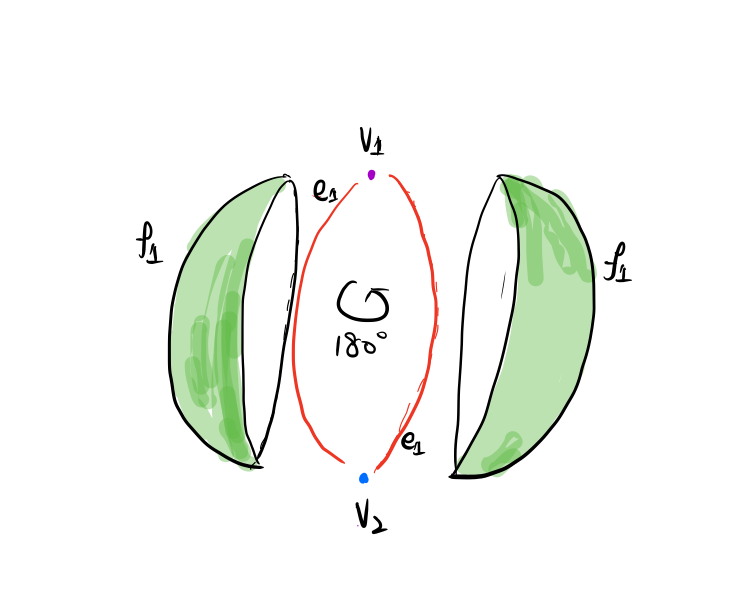
\includegraphics[scale=0.35]{Rotation GCW.png}\]

\end{example}
\end{tcolorbox}


\begin{tcolorbox}[colback=yellow!5!white,colframe=yellow!30!white]
\begin{example}
    Let $G=C_2$ acting on $S^2$ by the antipodal map, given by the figure below. It has a $G$-CW structure given by the following cells: 

    \begin{itemize}
        \item $1$ zero-cells $v_1$ of the form $C_2/C_2\times *$, which are the poles  corresponding to the fixed points of the $C_2$ action;
        \item $1$ one-cell $e_1$ of the form $C_2/e\times D^1$, which are the two great circles $e_1$ joining the poles;
        \item $1$ two-cell $f_1$ of the form $C_2/C_2\times D^2$, which are the two hemispheres. 
    \end{itemize}

    \[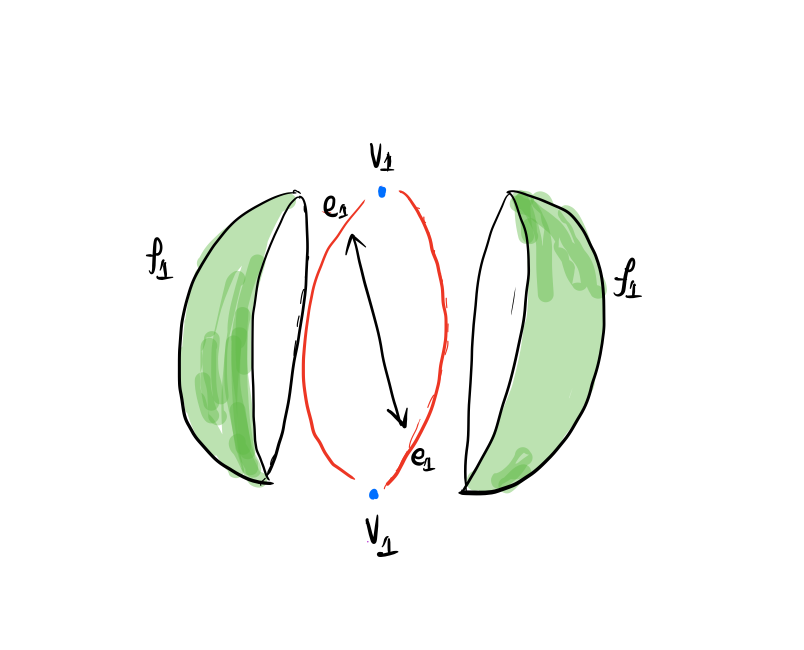
\includegraphics[scale=0.35]{antipodal.png}\]
\end{example}
\end{tcolorbox}


\begin{tcolorbox}[colback=purple!5!white,colframe=purple!75!black]
\begin{definition}
Let $H$ be a subgroup of $G$. Define $\pi_n^H(X):=\pi_n(X^H)$. A map $f: X\to Y$ of $G$-spaces is a \underline{\textbf{weak equivalence}} if for all subgroups $H\subset G$,
\[f_*:\pi_n^H(X)\to \pi_n^H(Y)\]
is an isomorphism. 
\end{definition}
\end{tcolorbox}

Let $\textbf{GTop}$ be the category of $G$-spaces and $G$-maps. There is a cofibrantly-generated model structure that we can put on $\textbf{GTop}$:

\begin{tcolorbox}[colback=red!5!white,colframe=red!30!white]
\begin{theorem}
\label{Fine-model}
    There is a cofibrantly-generated model structure on $\textbf{GTop}$, given by 
    \begin{enumerate}
        \item A $G$-map $f:X\to Y$ is a fibration iff for all $H\subset G$, $f^H: X^H\to Y^H$ is a fibration.
        \item A $G$-map $f:X\to Y$ is a weak equivalence iff for all $H\subset G$, $f^H: X^H\to Y^H$ is a weak equivalence. 
    \end{enumerate}
\end{theorem}
\end{tcolorbox}
An immediate consequence of the model category structure is the equivariant Whitehead's Theorem

\begin{tcolorbox}[colback=green!5!white,colframe=green!30!white]
\begin{corollary}
Let $f: X\to Y$ be a weak equivalence of cofibrant-fibrant objects in a model category. Then, $f$ is a homotopy equivalence. In particular, every object in $\textbf{GTop}$ is fibrant, and $G$-CW complexes are  cofibrant. 
\end{corollary}
\end{tcolorbox}

\subsection{Elmendorf's Theorem}
From the model structure given in Theorem \ref{Fine-model}, we have a vague sense of the following ``equivalence":
\[\textrm{G-homotopy type of } X\Leftrightarrow \{ \textrm{ordinary homotopy type of } X^H:H\subset G \}\]
And Elmendorf's Theorem will make the equivalence precise. We start by introducing the orbit category:

\begin{tcolorbox}[colback=purple!5!white,colframe=purple!75!black]
\begin{definition}
The \underline{\textbf{orbit category}} $\mathcal{O}_G$ is the full subcategory of $\textbf{GTop}$ on the objects $\{G/H: H\leq G\}$.
\end{definition}
\end{tcolorbox}
The following lemma will make the structure of $\mathcal{O}_G$ clearer.

\begin{tcolorbox}
\begin{lemma}
\label{equihom}
$\textrm{Map}^G(G/H,G/K)\cong (G/K)^H$
\end{lemma}
\end{tcolorbox}
\begin{proof}
    Note that there exists a $G$-equivariant maps $\varphi: G/H\to G/K$, determined by $\varphi(H)=gK$ iff $gHg^{-1}\subseteq K$ iff $h(gK)=gK$ for all $h\in H$. 
\end{proof}


\begin{tcolorbox}[colback=yellow!5!white,colframe=yellow!30!white]
\begin{example}
The orbit category for a finite cylic group $C_p$ is given by 
\[\begin{tikzcd}
	{C_p/e} \\
	{C_p/C_p}
	\arrow["{C_p}", from=1-1, to=1-1, loop, in=55, out=125, distance=10mm]
	\arrow["{\textrm{collapse}}", from=1-1, to=2-1]
\end{tikzcd}\]
\end{example}
\end{tcolorbox}

Let $\textrm{Fun}(\mathcal{O}_G^{op},\textbf{Top})$ be the functor category of contravariant functors from $\mathcal{O}_G$ to the category of topological spaces. We have the following fact on the model structure on functor categories:

\begin{tcolorbox}[colback=red!5!white,colframe=red!30!white]
\begin{theorem}
Let $\mathcal{D}$ be a model category and $\mathcal{C}$ be a cofibrantly generated model category. Then, $\textrm{Fun}(\mathcal{C},\mathcal{D})$ admits a model structure. 
\end{theorem}
\end{tcolorbox}

It is useful to know that the weak equivalences in $\textrm{Fun}(\mathcal{O}_G^{op},\textbf{Top})$ is given pointwise: a natural transformation $\eta: \mathcal{F}\to \mathcal{G}$ is a weak equivalence iff $\eta_{G/H}:\mathcal{F}(G/H)\to \mathcal{G}(G/H) $ is a weak equivalence. 



\begin{tcolorbox}[colback=purple!5!white,colframe=purple!75!black]
\begin{definition}
\label{thetafunctor}
There is a functor $\psi: \textbf{GTop}\to \textrm{Fun}(\mathcal{O}_G^{op},\textbf{Top})$ given by 
\[X\to (G/H\mapsto X^H)\]
\end{definition}
\end{tcolorbox}
It is easy to check the functoriality. Note that if we restrict to the subcategory $\psi$ to $\mathcal{O}_G$, the functor is just the Yoneda embedding: 
\[\textrm{Hom}_{\mathcal{O}_G}(G/-,G/K)=\textrm{Map}^G(G/-,G/K)\cong (G/K)^-\] 
as in lemma \ref{equihom}.

\begin{tcolorbox}[colback=blue!5!white,colframe=blue!30!white]
    \begin{proposition}
    There is a funcor $\theta: \textrm{Fun}(\mathcal{O}_G^{op},\textbf{Top})\to \textbf{GTop}$, which is left adjoint to the functor $\psi$ defined in definition \ref{thetafunctor}.
    \end{proposition}
    \end{tcolorbox}
    The functor $\theta$ is given by $X\mapsto X(G/e)$, where $X(G/e)$ is equipped with the following $G$-action: note that every $g\in G$ defines an $G$-map $G/e\to G/e$, which we denote by $R_g$.\[g\cdot x=X(R_g)(x)\] 

    It is easy to check that $(\theta,\psi)$ is an adjoint pair. In fact, more can be said:
    
    \begin{tcolorbox}[colback=red!5!white,colframe=red!30!white]
        \begin{theorem}[Elmendorf, 83]
         $\textrm{Fun}(\mathcal{O}_G^{op},\textbf{Top})$ and $\textbf{GTop}$ have isomorphic homotopy category. 
        \end{theorem}
        \end{tcolorbox}
    The original proof due to Elmendorf constructs the equivalence explicitly using the Bar construction to obtain a homotopy inverse to the embedding $\psi$. The theorem can also be put into a more modern framework with the development of model categories (we can even promote this to the infinity categories setting):

    \begin{tcolorbox}[colback=red!5!white,colframe=red!30!white]
    \begin{theorem}
    $(\theta,\psi)$ is an Quillen equivalence of model categories.
    \end{theorem}
    \end{tcolorbox}

\subsection{Bredon Cohomology}  
The goal is to construct a cohomology theory satisfying the Eilenberg-Steenrod axioms under the equivariant setting. The original construction of this is due to G. Bredon given in \cite{Bredon}.
 \begin{tcolorbox}[colback=purple!5!white,colframe=purple!75!black]
 \begin{definition}
 (Equivariant generalized cohomology) Let $G\textbf{CW}_*$ be the category of pointed $G$-CW complexes with equivariant maps. Then, a generalized cohomology theory on $G\textrm{CW}_*$ is a sequence of contravariant functors 
 \[\tilde{H}^n:=G\textbf{CW}_*\to \textbf{Ab} \]
 satisfying the following:
 \begin{enumerate}
    \item if $f,g$ are equivariantly homotopic, then $\tilde{H}^n(f)=\tilde{H}^n(g)$.
    \item There exists a sequence of natural isomorphisms
   \[\tilde{H}^n(X)\to \tilde{H}^{n+1}(S^1\wedge X)\]
   where $G$ acts trivially on $S^1$ in the smash. 
    \item The sequence 
    \[\tilde{H}^n(X/A)\to \tilde{H}^n(X)\to \tilde{H}^n(A)\]
    is exact.
 \end{enumerate}
 \end{definition}
 \end{tcolorbox}

\begin{tcolorbox}[colback=green!5!white,colframe=green!30!white]
\begin{remark}
The above axioms is built upon pointed ``single" spaces. It is in fact equivalent to the usual theory built upon pairs, and is justified in \cite{WH}.
\end{remark}
\end{tcolorbox}
For a non-equivariant reduced generalized cohomology theory $\tilde{h}^*$, the Atiyah-Hirzebruch spectral sequence tells us that the coefficients groups $\tilde{h}^*(pt)$ basically determines the cohomology theory on CW complexes. Heuristically, the cohomology is determined by the building blocks, which are contractible open cells. However, in the equivariant setting, the building blocks are more complicated: they are orbits of ordinary cell of the form $G/H\times D^n$. Thus, it makes sense to understand $\tilde{h}^*(G/H)$ for all $H$, and this will be our new ``coefficients." We are led to the following definition:

\begin{tcolorbox}[colback=purple!5!white,colframe=purple!75!black]
\begin{definition}
A \underline{\textbf{coefficient system}} is a contravariant functor $\mathcal{F}: \mathcal{O}_G\to \textrm{Ab}$.
\end{definition}
\end{tcolorbox}


\begin{tcolorbox}[colback=yellow!5!white,colframe=yellow!30!white]
\begin{example}
\label{ccs}
Fix an abelian group $N$. A \underline{\textbf{constant coefficient system}} $\mathcal{O}_G\to \textbf{Ab}$ is given by mapping all objects to $N$ and all morphisms to the identity. 
\end{example}
\end{tcolorbox}



Recall that if a reduced cohomology theory is called \underline{\textbf{ordinary}} if it satisfies the dimension axiom, i.e the zeroth reduced cohomology group (a.k.a the coeffcient system) is trivial on a point. Our goal now is to construct such a theory in the equivariant setting, which is called Bredon cohomology. 

Note that by the general theory of abelian categories, the functor category of coefficient systems $\mathcal{CS}:=\textrm{Fun}(\mathcal{O}_G, \textbf{Ab})$ is abelian. It is now possible to define Bredon cohomology on a $G$-CW complex by explicitly defining the cochain complexes on cells, similar to CW cohomology and done in \cite{Bredon}. However, we may package the cochains into the following form 

\begin{tcolorbox}[colback=purple!5!white,colframe=purple!75!black]
\begin{definition}
Fix an $G$-CW complex $X$. For each $n$, we may define a coefficient system $C_n(X)$ given by 
\[G/H\mapsto H_n((X^H)_{n},(X^H)_{n-1}; \mathbb{Z})=C_n^{CW}(X^H)\]
The differential of the CW chain complex induces a chain complex of coefficient systems $C_{\cdot}(-)$. 
\end{definition}
\end{tcolorbox}
Let us see how the definition makes sense: the $G$-CW structure (easy to check when $G$ finite) naturally induces a CW structure on all fixed point spaces $X^H$, for a G-CW cell breaks up into an orbit of ordinary CW cells in a way that respects glueing. Thus, each ordinary cell in $C^{CW}_n(X^H)$ can be viewed as an element in a $G/H$ orbit. For a morphism $G/H\to G/K$, we now have the induced morphism 
\[C_n^{CW}(X^K)\to C_n^{CW}(X^H)\]
given by $G$-action.

\begin{tcolorbox}[colback=purple!5!white,colframe=purple!75!black]
\begin{definition}
The \underline{\textbf{Bredon cohomology}} of $X$ with coefficients in a system $M$ is defined by 
\[H_G^n(X;M):=H^n(Hom_{\mathcal{CS}}(C_{\cdot}(X),M))\]
\end{definition}
\end{tcolorbox}

Similarly, we may define Bredon homology with coefficients: for singular homology, we are tensoring the chain complex with some abelian group; for coefficient systems, we have the analog of ``tensoring," which is a coend. We first recall the following construction


\begin{tcolorbox}[colback=green!5!white,colframe=green!30!white]
\begin{remark}
The tensor product of of a right $R$-module $A$ and a left $R$-module $B$ is the coequalizer of the diagram 
\[\alpha_A:\alpha_B: A\otimes R\otimes B\to A\otimes B\]
where the the tensor product is given in $\textbf{Ab}$ and the two maps are given by the $R$ action on $A,B$, respectively.
\end{remark}
\end{tcolorbox}

To distinguish a covariant coefficient system with a contravariant one, we give it another name
\begin{tcolorbox}[colback=purple!5!white,colframe=purple!75!black]
\begin{definition}
A covariant functor $N: \mathcal{O}_G\to \textbf{Ab}$ is called an \underline{$\mathcal{O}_G$\textbf{-module}}.
\end{definition}
\end{tcolorbox}

\begin{tcolorbox}[colback=purple!5!white,colframe=purple!75!black]
\begin{definition}
The \underline{\textbf{Bredon homology}} with coefficients an $\mathcal{O}_G$-module $N$ is defined to be the homology of the chain complex 
\[C_*(X)\otimes_{\mathcal{O}_G} N\]
where each degree $C_n(X)\otimes_{\mathcal{O}_G} N$ is defined to be the coequalizer of the following
\[ \bigoplus_{H,K\leq G}\bigoplus_{\textrm{Hom}_{\mathcal{O}_G}(G/H,G/K)}C_n(X)(G/K)\otimes N(G/H)\rightrightarrows \bigoplus_{H\leq G}C_n(X)(G/H)\otimes N(G/H) \]
where the two arrows are given by the contravariant functoriality of $C_n$ and covariant functoriality of $N$. The differentials are induced by the cellular differentials of $C_*(X)$.

\end{definition}
\end{tcolorbox}


\begin{tcolorbox}[colback=green!5!white,colframe=green!30!white]
\begin{remark}
The above construction is the \underline{\textbf{coend}}
\[C_n(X)\otimes_{\mathcal{O}_G} N=\int^{G/H\in \mathcal{O}_G}C_n(X)(G/H)\otimes_{\mathcal{O}_G} N(G/H)\]
\end{remark}
\end{tcolorbox}
One may unravel the definition of coequalizer and note that 
\[C_n(X)\otimes_{\mathcal{O}_G} N\cong \bigoplus_{H\leq G}C_n(X)(G/H)\otimes N(G/H)/\sim\]
where the equivalence relation is given by: for every $f\in \textrm{Hom}_{\mathcal{O}_G}(G/H,G/K)$, we have $f^*x\otimes y\sim x\otimes f_*y$ for every $x\otimes y\in C_n(X)(G/K)\otimes N(G/H)$.

\subsection{Computations}



\subsubsection{Constant Coefficients}
We start with a concrete example: let $\sigma: C_2\to GL_1(\mathbb{R})$ be the sign representation. Taking its direct sum with itself given us a two dimensional real $C_2$-representation $2\sigma$, which on coordinates is given by $(x,y)\mapsto (-x,-y)$. Then, taking the one-point compactification gives us a representation sphere, which we denote as $S^{2\sigma}$. The representation sphere has the following $G$-CW decomposition 
\[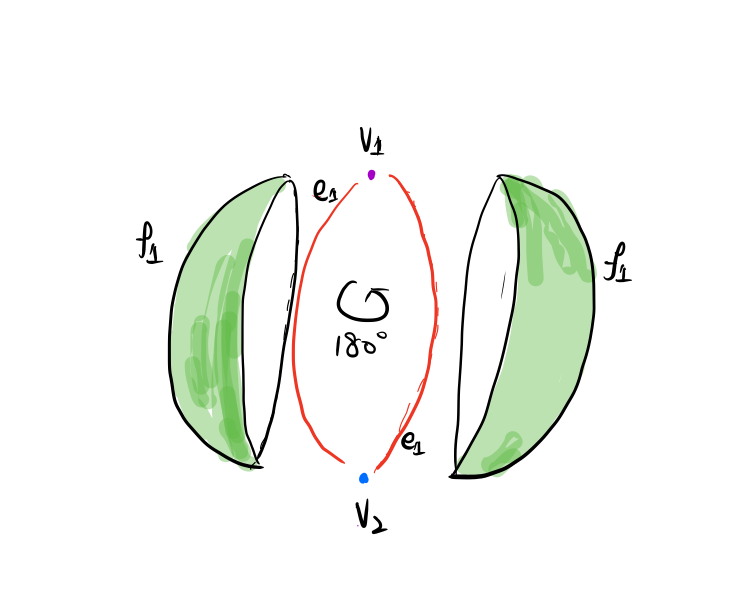
\includegraphics[scale=0.35]{Rotation GCW.png}\]

which is the same as in example \ref{2sigma} and we shall compute its Bredon cohomology with constant coefficient system $\underline{\mathbb{Z}}$, defined in example \ref{ccs}.

The orbit category of $C_2$ is easy to describe:
\[\begin{tikzcd}
	{C_2/e} \\
	{C_2/C_2}
	\arrow["{\textrm{swap}}", from=1-1, to=1-1, loop, in=55, out=125, distance=10mm]
	\arrow["{\textrm{collapse}}", from=1-1, to=2-1]
\end{tikzcd}\]
Then, the $n$th group in our chain complex, which is $\textrm{Hom}_{\mathcal{CS}}(C_n(X),\underline{\mathbb{Z}})$, is computed as follows: the zero cells are simply the two poles, which are fixed under the $G$-action. Thus, for $n=0$, we are looking for morphisms of the following diagram 
\[\begin{tikzcd}
	{C_2/e:} & {\mathbb{Z}v_1\oplus\mathbb{Z}v_2} && {\mathbb{Z}} \\
	{C_2/C_2:} & {\mathbb{Z}v_1\oplus\mathbb{Z}v_2} && {\mathbb{Z}}
	\arrow["Id", from=1-2, to=1-2, loop, in=55, out=125, distance=10mm]
	\arrow[dashed, from=1-2, to=1-4]
	\arrow["Id", from=1-4, to=1-4, loop, in=55, out=125, distance=10mm]
	\arrow["Id", from=2-2, to=1-2]
	\arrow[dashed, from=2-2, to=2-4]
	\arrow["Id", from=2-4, to=1-4]
\end{tikzcd}\]

It is clear that the morphism is determined by the what happens at the $C_2/e$ spot, and we have total freedom to send $v_1,v_2$ to whichever element we wish. Thus, $\textrm{Hom}_{\mathcal{CS}}(C_0(X),\underline{\mathbb{Z}})\cong \mathbb{Z}\oplus \mathbb{Z}$. 

For $n=1$, the story is a bit different: we have two $1$-cells, and the $G$-action swaps these two. The morphisms 
we are looking for morphisms of the following diagram 
\[\begin{tikzcd}
	{C_2/e:} & {\mathbb{Z}e_1\oplus\mathbb{Z}e_2} && {\mathbb{Z}} \\
	{C_2/C_2:} & 0 && {\mathbb{Z}}
	\arrow["Swap", from=1-2, to=1-2, loop, in=55, out=125, distance=10mm]
	\arrow[dashed, from=1-2, to=1-4]
	\arrow["Id", from=1-4, to=1-4, loop, in=55, out=125, distance=10mm]
	\arrow[from=2-2, to=1-2]
	\arrow[dashed, from=2-2, to=2-4]
	\arrow["Id", from=2-4, to=1-4]
\end{tikzcd}\]
To be compatible with the swap map, we see that $e_1,e_2$ must be mapped to the same element, thus $\textrm{Hom}_{\mathcal{CS}}(C_1(X),\underline{\mathbb{Z}})\cong \mathbb{Z}$. The story with $n=2$ is the same as $n=1$, and the Bredon cochain complex is then 
\[0\to \mathbb{Z}\varphi_1\oplus \mathbb{Z}\varphi_2\xrightarrow{d_0} \mathbb{Z}f\xrightarrow{d_1} \mathbb{Z}g\to 0\] 
It is easy to first \textcolor{red}{correctly compute} the cellular differential $d(e_1)=d(e_2)=v_1+v_2$, and $d(f_1)=f(f_2)=e_1-e_2$. It then follows that the induced differentials $d_0((\varphi_1,0))=d_0((0,\varphi_1))=f$, which also implies $d_1$ is the $0$-map. Thus, we have 
\[H^n_{\textrm{Bredon}}(S^{2\sigma}; \underline{\mathbb{Z}})=
\begin{cases}
    \mathbb{Z}& n=0,2\\
    0 & \textrm{otherwise}
\end{cases}
\] 

This procedure can be generalized: note that since we are taking the constant coefficient system, each $\textrm{Hom}_{\mathcal{CS}}(C_n(X),\underline{\mathbb{Z}})\cong \mathbb{Z}$ is determined by what happens at the $G/e$ level; the cell complex at $G/e$ level are freely generated by the $n$-cells under the $G$-action, which reduces to morphisms 
\[\begin{tikzcd}
	{\bigoplus_{\textrm{n-cells}}\mathbb{Z}} && {\mathbb{Z}}
	\arrow["G", from=1-1, to=1-1, loop, in=55, out=125, distance=10mm]
	\arrow[from=1-1, to=1-3]
\end{tikzcd}\]
so the morphisms is determined by where to send a $G$-orbit of $n$-cells. We then have the canonical identification 
 
 \begin{tcolorbox}[colback=red!5!white,colframe=red!30!white]
 \begin{theorem}
 If $X$ is a $G$-CW complex, and $G$ has a $CW$-decomposition induced from the $G$-CW structure (always hold when $G$ is finite), we have the canonical isomorphism 
\[\textrm{Hom}_{\mathcal{CS}}(C_n(X),\underline{\mathbb{Z}})\cong \textrm{Hom}_{\textbf{Ab}}(C_n(X)(G/e)/G,\mathbb{Z})\]. As a corollary, we also have the isomorphism:
 \[H^*_{\textrm{Bredon}}(X;\underline{\mathbb{Z}})\cong H^*_{\textrm{CW}}(X/G;\mathbb{Z})\]
 \end{theorem}
 \end{tcolorbox}
There is a similar statement for homology:

 
\begin{tcolorbox}[colback=red!5!white,colframe=red!30!white]
    \begin{theorem}
    If $X$ is a $G$-CW complex, and $G$ has a $CW$-decomposition induced from the $G$-CW structure (always hold when $G$ is finite), we have the canonical isomorphism 
   \[C_n(X)\otimes_{\mathcal{O}_G}\underline{\mathbb{Z}}\cong C_n(X)(G/e)/G\otimes \mathbb{Z}\]. As a corollary, we also have the isomorphism:
    \[H_*^{\textrm{Bredon}}(X;\underline{\mathbb{Z}})\cong H_*^{CW}(X/G; \mathbb{Z})\]
    \end{theorem}
    \end{tcolorbox}


\begin{tcolorbox}[colback=yellow!5!white,colframe=yellow!30!white]
\begin{example}
Consider the Bredon homology of $S^{2\sigma}$ with coefficients $\underline{\mathbb{Z}}$. By Theorem $1.7$, this reduces to the computation of the cellular homology of $S^{2\sigma}/C_2\cong S^2$, 
\[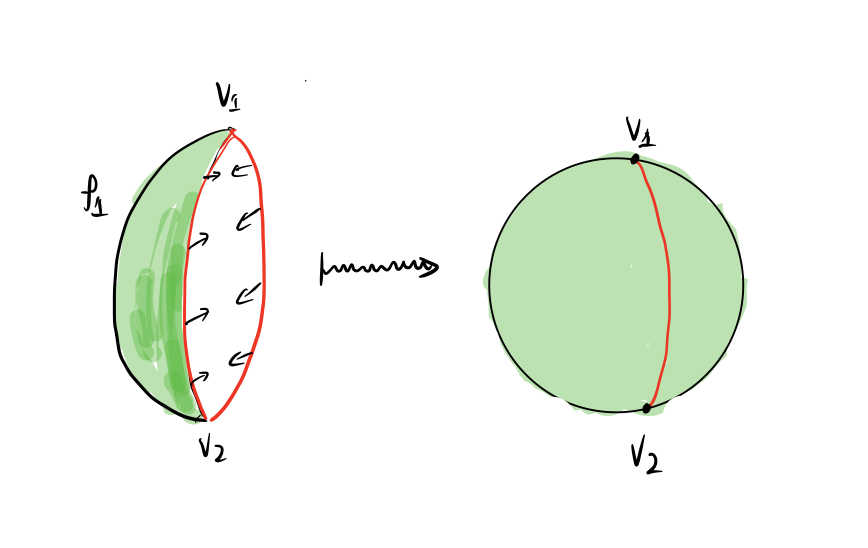
\includegraphics[scale=0.35]{mod c2.png}\]
which is concentrated in degree $0,2$. The generalization holds for $S^{n\sigma}$
\[H_k^{\textrm{Bredon}}(S^{n\sigma}; \underline{\mathbb{Z}})=
\begin{cases}
    \mathbb{Z} & k=0,n\\
    0 & \textrm{otherwise}.
\end{cases}\]
\end{example}
\end{tcolorbox}

\subsubsection{Free Action} 
Now let fix some arbitrary coefficients system ($\mathcal{O}_G$-module) $\underline{M}$. It turns out that if the $G$-action on a $G$-CW complex is free, then the Bredon (co)homology also reduces to cellular homology. We outline the proof for cohomology: suppose the $G$-action on $X$ is free, then the group $C_n(X)(G/H)$ is trivial for all subgroups $H$ except for $H=e$. Again, we reduce computing $\textrm{Hom}_{\mathcal{CS}}(C_n(X),\underline{M})$ reduces to morphisms at $G/e$ level.

\[\begin{tikzcd}
	{C_n(X)(G/e)} && {\underline{M}(G/e)}
	\arrow["G", from=1-1, to=1-1, loop, in=55, out=125, distance=10mm]
	\arrow[dashed, from=1-1, to=1-3]
	\arrow["G", from=1-3, to=1-3, loop, in=55, out=125, distance=10mm]
\end{tikzcd}\]
Note that each $C_n(X)(G/e)$ is freely generated by the $n$-cells of $X$, and it has the free $G$-action. Moreover, a morphism of the diagram is equiavalent to specifying a morphism $\mathbb{Z}\to M(G/e)$ for each orbit of the $G$-action, and we have (possibly non-canonically), that 
\[\textrm{Hom}_{CS}(C_n(X),\underline{M})\cong \textrm{Hom}(C_n(X)/G,M(G/e))\]
It follows that 

\begin{tcolorbox}[colback=red!5!white,colframe=red!30!white]
\begin{theorem}
If $G$ acts freely on $X$, we have 
\[H^*_{\textrm{Bredon}}(X;\underline{M})\cong H^*_{CW}(X/G;M(G/e))\]
and the similar statement for homology holds as well. 
\end{theorem}
\end{tcolorbox}


\begin{tcolorbox}[colback=yellow!5!white,colframe=yellow!30!white]
\begin{example}
Consider the unit sphere $S(n\sigma)$ in the $n$-dimensional $C_2$ representation given by the $n$-times direct sum of the sign representation. The induced $C_2$-action on $S(n\sigma)$ is the antipodal action. Thus, 
\[H_{\textrm{Bredon}}^*(S(n\sigma); \underline{M})\cong H^*(S(n\sigma)/C_2;M(C_2/e))\cong H^*(\mathbb{RP}^{n-1};M(C_2/e))\]
and we know how to compute the cohomology of real projective space. 
\end{example}
\end{tcolorbox}








\subsection{Classical Application}
Here are two questions we may ask: given a finite $p$-group $G$ acting on $X$, can we recover the cohomology of $X^G$ based on the cohomology of $X$, while somehow incoporating the $G$-action? The second point of interest is the Sullivan conjecture: the study of \'etale homotopy theory allows one to determines algebraically the profinite completion of a variety from its \'etale homotopy type. The same situation occurs as before: given a variety $V$ over the complex numbers, there is a natural $\mathbb{Z}/2$-action on the variety, with $V^G=V(\mathbb{R})$. How much can we say about $V(\mathbb{R})$ if we are given the \'etale homotopy type of $V$ and the $G$-action? In this case, the fixed points is not a homotopy invariant, so we should consider the homotopy fixed points instead, and the sullivan conjecture states that 


\begin{tcolorbox}[colback=red!5!white,colframe=red!30!white]
\begin{theorem}
(Sullivan Conjecture) $V(\mathbb{C})^{\mathbb{Z}/2}\to V(\mathbb{C})^{h \mathbb{Z}/2}$ becomes an isomorphism after $2$-adic completion. More generally, let $G$ be a finite $p$-group, then $X^G\to X^{hG}$ becomes an equivalence after $p$-adic completion. 
\end{theorem}
\end{tcolorbox}
This is a difficult problem which is resolved by Haynes Miller in 1984, whose problem goes beyond the tools already developed in the notes. However, one possible application is a quick proof of a theorem by Smith: 

\begin{tcolorbox}[colback=red!5!white,colframe=red!30!white]
\begin{theorem}
    Let $G$ be a finite $p$-group and $X$ be a finite $G$-CW complex such that (the underlying topological space of) $X$ is an $p$-cohomology sphere.16 Then, $X^G$ is either empty or an $p$-cohomology sphere of smaller dimension.
\end{theorem}
\end{tcolorbox}
A proof of this can be found in \cite{ST}.







\section{Spectra and the Stable Category}
\subsection{Motivations}
So why do we want spectra? The first motivation is Brown Reresentability Theorem, which is about represeting reduced cohomology theories 

\begin{tcolorbox}[colback=red!5!white,colframe=red!30!white]
\begin{theorem}[Brown Representability Theorem]
Let $\tilde{h}^*$ be a reduced cohomology theory on pointed CW-complexes. Then, for each $n\in \mathbb{Z}$, there exists a connected pointed CW complex $K_n$ such that 
\[\tilde{h}^n(X)\cong [X,K_n]\]
for all $n$. Moreover, the $K_n$ are determined up to homotopy equivalence. 
\end{theorem}
\end{tcolorbox}
In fact, there are more structure to the set $\{K_n\}$: using the suspension axiom and loop-suspension adjunction, we see that there must be an isomorphism 
\[[X,K_n]\cong \tilde{h}^n(X)\cong \tilde{h}^{n+1}(\Sigma X)\cong [\Sigma X,K_n]\cong [X,\Omega K_n]\]
Taking $X$ to be $K_n$, we note that the indetitiy map from the LHS corresponds uniquely to a map $\alpha_n: K_n\to \Omega K_n$, which we will call the \underline{\textbf{structure map.}}. By naturality and taking $A=S^k$, the structure map induces a weak equivalence 
\[K_n\cong  \Omega K_n\]
. This motivates the definintion for $\Omega$-Spectra

\begin{tcolorbox}[colback=purple!5!white,colframe=purple!75!black]
\begin{definition}
A $\underline{\textbf{spectrum}}$ is a sequence of pointed topological spaces $\{X_n\}$ with $\underline{\textbf{structure maps}}$.
\[\Sigma X_n\to X_{n+1}\]
. An \underline{\textbf{$\Omega$ spectrum}} is a spectrum whose adjoint structure maps
\[X_n\to \Omega X_{n+1}\]
are weak equivalences. 
\end{definition}
\end{tcolorbox}
So we see that a reduced cohomology theory corresponds to an $\Omega$-spectrum. In fact, it is not hard to show that an $\Omega$-spectrum defines a reduced cohomology theory as well. We can then present Brown Representability Theorem in the following way:
\begin{tcolorbox}[colback=red!5!white,colframe=red!30!white]
\begin{theorem}[Brown Representability Theorem]
    Every reduced cohomology theory on the category of basepointed CW complexes  has the form $\tilde{h}^n(X) = [X,K_n]$ for some $\Omega$-spectrum $\{K_n\}$
\end{theorem}
\end{tcolorbox}

\begin{tcolorbox}[colback=yellow!5!white,colframe=yellow!30!white]
\begin{example}[Eilenberg-Maclane Spectrum]
The $\Omega$-spectrum that represents reduced ordinary cohomology with coefficients in $\mathbb{Z}$ is given by the $\Omega$-spectra that is the Eilenberg-Maclane spaces $HG:=\{K(G,n)\}$.
\end{example}
\end{tcolorbox}

\begin{tcolorbox}[colback=yellow!5!white,colframe=yellow!30!white]
\begin{example}
    The $\Omega$-spectrum that represents reduced complex topological $K$-theory is given by $\{KU_n\}$, where 
    \[  KU_n=
    \begin{cases}
        BU\times \mathbb{Z}& $n$-\textrm{even}\\
        \Omega BU & $n$-\textrm{odd}
    \end{cases}\]
  In particular, Bott-periodicity shows that the structure maps are weak-equivalences.
\end{example}
\end{tcolorbox}

Here is a natural question: how do we design a category of spectra, such that an "equivalence" if spectra will give equivalent reduced cohomology theories?

The second motivation is stable homotopy groups and stable maps. The heuristics is: in most cases the homotopy classes of maps $[X,Y]$ is very difficult to compute. However, the stable maps $\varinjlim_n[\Sigma^nX,\Sigma^n Y]$ gives us nice approximation and is sometimes easier to understand. Spanier-Whitehead duality is a nice example of this (Theorem $2.5$). 


\begin{tcolorbox}[colback=purple!5!white,colframe=purple!75!black]
\begin{definition}
Let $X$ and $Y$ be pointed CW-complexes. The set of $\underline{\textbf{stable homotopy classes of maps}}$ from $X$ to $Y$ is defined to be 
\[[X,Y]^s:= \varinjlim_{k}[\Sigma^k X, \Sigma^k Y] \]
\end{definition}
\end{tcolorbox}
One form of the Freudenthal suspension theorem says that if $Y$ is $n$-connected and $X$ has dimension less than $2n+1$, then the suspension map $[X,Y]\to [\Sigma X,\Sigma Y]$ is bijective. In this case, we see that the colimit actual stablizes after at a finite stage. 

\begin{tcolorbox}[colback=purple!5!white,colframe=purple!75!black]
\begin{definition}
For a pointed CW-complex, the $n$-th \underline{\textbf{stable homotopy group}} is defined to be 
\[\pi_n^{st}(X):=\varinjlim_{k}\pi_{n+k}(\Sigma^k X)=\varinjlim_{k}[\Sigma^k S^n, \Sigma^k X]=[S^n,X]^s\]
\end{definition}
\end{tcolorbox}
By definition, we see that the stable homotopy group should be the homotopy group in some "stable category". Moreover, stable homotopy groups actually defines a reduced homology theory: the two axioms that are not trivial are the LES and the wedge axiom. The key point is that Blaker's Massey Theorem plus the LES of homotopy groups of a pair will give us the LES of stable homotopy groups of a pair; the wedge axiom follows from that $\Sigma^i X\wedge \Sigma^i Y$ is the $2i-1$ skeleton of  $\Sigma^i X\times \Sigma^i Y$. Generalizing this, we have 

\begin{tcolorbox}[colback=red!5!white,colframe=red!30!white]
\begin{theorem}
    Let $K$ be a CW-complex. The sequence $h_i(X) = \pi^s_i(X \wedge K)$ forms a reduced homology theory on the category of basepointed CW-complexes and basepoint-preserving maps.
\end{theorem}
\end{tcolorbox}

We can also define the homotopy groups of a spectrum as a generalization:

\begin{tcolorbox}[colback=purple!5!white,colframe=purple!75!black]
\begin{definition}[Homotopy groups of a spectrum]
Suppose $K=\{K_i\}$ is a spectrum. Then, 
\[\pi_n(K):=\varinjlim \pi_{n+i}(K_i)\]
where the inductive limit is induced by the suspension structure maps. 
\end{definition}
\end{tcolorbox}

\begin{tcolorbox}[colback=yellow!5!white,colframe=yellow!30!white]
\begin{example}
Given a topological space $X$, we have the associated \underline{\textbf{suspension spectrum}} $\Sigma^{\infty}X=\{\Sigma^kX\}$. Then, the stable homotopy groups of $X$ is given by the homotopy groups of its associated suspension spectrum. 
\end{example}
\end{tcolorbox}

\begin{tcolorbox}[colback=purple!5!white,colframe=purple!75!black]
\begin{definition}
Given a spectrum $K=\{K_n\}$ and a CW complex $X$, there is a associated smash spectrum $K\wedge X$, where $(K\wedge X)_n=K_n\wedge X$. The structure maps is given by 
\[\Sigma (K\wedge X)_n =\Sigma K_n\wedge X\to K_{n+1}\wedge X=\Sigma (K\wedge X)_{n+1}\]
\end{definition}
\end{tcolorbox}

\begin{tcolorbox}[colback=blue!5!white,colframe=blue!30!white]
\begin{proposition}
Let $K$ be a spectrum. Given a CW complex $X$, the sequence
\[h_n:=\pi_n(X\wedge K)\]
is a reduced homology theory.
\end{proposition}
\end{tcolorbox}
The proof mostly follows from the same tactics in proving the stable homotopy groups being a reduced homology theory.
\begin{tcolorbox}[colback=yellow!5!white,colframe=yellow!30!white]
\begin{example}[Singular homology]
If $K=HG$ is the Eilenberg-Maclane spectrum, then $h_i(X):=\pi_i(X\wedge K)$ is isomorphic to singular homology with coefficients in $G$. We only have to check the dimension axiom 
\[h_i(S^0):=\varinjlim_n \pi_{n+i}(K(G,n))\]
which is trivial except $i=0$. 
\end{example}
\end{tcolorbox}


Thus, we have seen that the singular homology is recovered from a spectrum; moreover, a spectrum gives a reduced homology theory by proposition $2.3.1$. 


\subsection{Duality}
We now have spectra and stable morphisms that represents cohomology and homology. Moreover, we want to recover some of the classical duality theorems in the case of singular (co)homology. 

\begin{tcolorbox}[colback=red!5!white,colframe=red!30!white]
\begin{theorem}[Alexander Duality]
If $K$ is a compact, locally contractible, nonempty, proper subspace of $S^n$. Then we have the isomorphism
\[\tilde{H}^{n-i-1}(K;\mathbb{Z})\cong \tilde{H}_i(S^n-K;\mathbb{Z})\] 
\end{theorem}
\end{tcolorbox}
The theorem in particular implies that different embeddings of some nice enough space in $S^n$ has isomorphic homology. However, they do not necessarily have the same homotopy type, as there are tons of examples in knot theory. Nevertheless, Spanier and Whitehead prove the following theorem, which states that the homotopy types are the same after sufficiently many suspensions. 

\begin{tcolorbox}[colback=red!5!white,colframe=red!30!white]
\begin{theorem}[Spanier-Whitehead Duality]
    Let $X$ be a compact simplicial complex. Let $f,g: X\to S^n$ be two simplicial embeddings. Then for some sufficiently large $M$ the $M$-fold suspensions $\Sigma^M (S^n\setminus f(X))$ and $\Sigma^M (S^n\setminus g(X))$ are homotopy equivalent.
\end{theorem}
\end{tcolorbox}
To study this phenomenon more formally, Spanier-Whitehead proposed the now-called Spanier-Whitehead category:


\begin{tcolorbox}[colback=purple!5!white,colframe=purple!75!black]
\begin{definition}[Spanier-Whitehead Category]
The \underline{\textbf{Spanier-Whitehead category}}, or \underline{\textbf{$S$-category}} for short, has objects pairs $(X,n)$, where $X$ is a pointed finite CW complex, and $n$ is an integer. The morphisms are defined by 
\[Hom_{S}((X,n),(Y,m)):=\varinjlim_{q\geq \textrm{max}(|m|,|n|)}[\Sigma^{q+n} X, \Sigma^{q+m} Y]\]
\end{definition}
\end{tcolorbox}
We can think of $(X,m)$ as the $m$-fold suspension of $X$. If $m=n=0$, we see that $\textrm{Hom}_S((X,0),(Y,0))=\varinjlim_{k}[\Sigma^k X, \Sigma^k Y]$, which are simply the stable morphisms and that the different embeddings $X\to S^n$ become actually isomorphic in this category by theorem $2.5$. If $m>0$, we may denote $(X,-m)$ as $\Sigma^{-m}X$ to represent formal desuspensions. We can also think of this as "inverting smashing with spheres".


\begin{tcolorbox}[colback=purple!5!white,colframe=purple!75!black]
\begin{definition}
Let $\mathcal{C}$ be a symmetric monoidal category with the tensor product denoted by $\wedge$, and unit object $S^0$. Then, $X,Y$ are \underline{\textbf{dual}} if there are morphisms $X\wedge Y\to S^0$ and $S^0\to Y\wedge X$ such that the following compositions
\[X\cong X\wedge S^0\to X\wedge Y\wedge X\to S^0\wedge X\cong X\]
\[Y\cong S^0\wedge Y\to Y\wedge X\wedge Y\to Y\wedge S^0\cong Y\]
are the indetitiies in the symmetric monoidal category. Given an object $A$ in $\mathcal{C},$ we denote its dual as $DA$, if it exists.
\end{definition}
\end{tcolorbox}
Note that the definition implies precisely the adjunction 
\[\textrm{Hom}_{\mathcal{C}}(X\wedge A, Y)\cong \textrm{Hom}_{\mathcal{C}}(X, DA\wedge Y)\]. 



By the identity $\Sigma(X\wedge Y)\cong X\wedge \Sigma Y$, we see that the smash product defined by 
\[(X,m)\wedge (Y,n):=(X\wedge Y,m+n)\]
endows the $S$-category with a symmetric monoidal structure, with $S^0$ being the unit. Let us see some explicit dualities

\begin{tcolorbox}[colback=yellow!5!white,colframe=yellow!30!white]
\begin{example}
    $S^n$ is dual to $S^{-n}$, the formal $n-$fold desuspension of $S^0$. This follows directly from definition.
\end{example}
\end{tcolorbox}

\begin{tcolorbox}[colback=yellow!5!white,colframe=yellow!30!white]
    \begin{example}[Alexander duality in $S$-category]
   Let $X$ be a compact finite CW complex with an embedding $X\to S^{n+1}$. Let us denote the complement $S^n\setminus X$ as $D_nX$. Then, one may construct a map $X\wedge D_nX\to S^n$, and a desuspension of such map exhibits $X$ and $\Sigma^{-n}D_nX$ as duals. \\

   Let $Y$ be a finite discrete set of points. Then, $Y$ embeds in $S^1$, and the complement is homotopy equivalent to $Y$ again. This shows that $Y$ is self-dual. This example will come up later when we deal with finite $G$-sets and equivariant embeddings. 
    \end{example}
    \end{tcolorbox}


\begin{tcolorbox}[colback=yellow!5!white,colframe=yellow!30!white]
\begin{example}[Atiyah Duality]
Suppose $M$ is a closed smooth manifold with a smooth embedding $M\to \mathbb{R}^n$. Let $Tv$ be the Thom space of the normal bundle of the embedding. The Pontrjagin-Thom construction yields a map 
\[Tv\wedge M_+\to \Sigma^nM_+\xrightarrow{\textrm{collapse } M_+}S^n\]
which exhibits $Tv$ and $\Sigma^{-n}M_+$ as duals.
\end{example}
\end{tcolorbox}


\begin{tcolorbox}[colback=yellow!5!white,colframe=yellow!30!white]
\begin{example}[Poincar\'e Duality]
Let $M$ be a closed orientable manifold of dimension $m$, with an embedding in $M\to \mathbb{R}^n$. Let $H \mathbb{Z}$ be the Eilenberg-Maclane spectra that represents singualar cohomology. From Atiyah duality, we have $[DM,H \mathbb{Z}]\cong [S^0, M_+\wedge H \mathbb{Z}]=: \tilde{H}_*(M_+)$. On the other hand, $[DM, H \mathbb{Z}]=[\Sigma^{-n}Tv, H \mathbb{Z}]\cong \tilde{H}^{*}(\Sigma^{-n}Tv)$. By Thom isomorphism and suspension isomorphism
\[\tilde{H}^*(M_+)\cong \tilde{H}^{*+(n-m)}(Tv)\cong \tilde{H}^{*-m}(\Sigma^{-n}Tv)\]
and we establish the classical Poincar\'e duality $\tilde{H}^*(M_+)\cong \tilde{H}_{*-m}(M_+)$.
\end{example}
\end{tcolorbox}










\subsection{The Desired Stable Homotopy Category}
Building upon the motivations in the previous section, we want to build a category $\mathcal{SHC}$ that captures the stable phenomena and cohomology theories/homology theories. In particular, we want it to satisfy the following properties (not necessarily axioms):
\begin{enumerate}
    \item There is a functor $\Sigma^{\infty}: \textrm{HoTop}_*\to \mathcal{SHC}$, together with an adjoint $\Omega^{\infty}: \mathcal{SHC}\to \textrm{HoTop}_*$. \\
    \textcolor{blue}{The motivation for this is the suspension spectrum}.
    \item Let $A,B$ be CW complexes, where $A$ has finite dimension. Then, there is a natural isomorphism
    \[[\Sigma^{\infty}A, \Sigma^{\infty}B]\cong [A,B]^s\]
    \textcolor{blue}{The motivation for this is to capture stable morphisms}.
    \item The morphisms of $\mathcal{SHC}$ has the structure of graded abelian groups, with bilinear composition. We denote that graded components as $[-,-]_*$. Moreover, given a reduced cohomology theory $E^*$ there exists an object $K$ in $\textrm{Sp}$ such that 
    \[E^*(A)\cong [\Sigma^{\infty}A, K]_{-*}\]
    \textcolor{blue}{The motivation for this is to represent cohomology theories}.\\
    \item For every object $K$ in $\mathcal{SHC}$, one defines a reduced homology theory via 
    \[E_n(A):=\pi(K\wedge A)\]
    \textcolor{blue}{The motivation for this is to deterime homology theories}.
    \\
    \item $\mathcal{SHC}$ has a closed symmetric monoidal structure, with $\wedge$ as the tensor product and $F(-,-)$ as internal hom. The object $\Sigma^{\infty}S^0$ is the identity object.\\
    \textcolor{blue}{The motivation for this is that smashing with the suspension funcor induces isomorphism of stable homotopy groups, so it should induce an equivalence of spectra. The tensor-hom adjunction is going to help set up duality statements similar to Spanier-Whitehead duality and Poincar\'e duality.}.
\end{enumerate}
In particular, property $6$ was the central one in the sense that the entire theory began with the work of Spanier and Whitehead with their search for a category where one has the desired dualities in homotopy theory. It is also the structure that seems to be the hardest to obtain.  



\subsection{Attempts}

\subsubsection{The Spanier-Whitehead Category}
The first attempt to construct such a category is the Spanier-Whitehead category, where the objects are finite CW complexes, and the morphisms are stable maps. The catgeory was originally set up to perform Spanier-Whitehead duality (chronologically it was ), but the objects "almost" represents cohomology theories. We use the word almost because since the objects are only finite complexes, we do not have arbitrary products and coproduts, and the wedge axiom do not hold. 
\subsubsection{An Attempt for \textrm{Sp}}
By Brown representability, it should be natural to consider a category with objects spectra, and the natural choice for morphisms between spectra is a collection of level-wise maps that is compatible with the structure maps. A natural candidate for homotopies in this category is a map $H: X\wedge I_{+}\to Y$ However, it turns out there are not enough maps in this category, such that non-homotopy equivalent spectra might represent isomorphic cohomology theories. Adams then in his 74 paper resolves the issue by consider equivalences classes of "cofinal spectra," which turns out to be quite a complicated a construction. 

\subsubsection{\textrm{Ho(Sp)} and Structured Spectra}
The first construction in line with modern treatment of the subject is Bousfield and Friedlander's construction, which puts a model structure on the naive category of spectra, and considers its homotopy category. This category turns out satisfies all the properties that people wanted, and is referred to as the stable homotopy category.

However, people still searched for a point-set model that does so without going through the homotopy category. The sad news is Lewis in 91 showed that it is impossible to put a symmetric monoidal structure on the category of spectra that also satifies a list of desirable axioms. Nevertheless, people later constructed models category categories of structured spectra, such as orthogonal spectra and symmetric spectra, whose homotopy category is equivalent to the stable homotopy category. Point-set wise, although they do not satisfies all of the desired properties, they are at least symmetric monoidal, and their additional structure turn out to be incredibly useful.

\subsection{Orthogonal Spectra}

\begin{tcolorbox}[colback=purple!5!white,colframe=purple!75!black]
\begin{definition}
An \underline{\textbf{orthogonal spectrum}} consists of the following data:
\begin{enumerate}
    \item A sequence of pointed topological spaces $X_n$
    \item A basepoint-preserving left $O(n)$-action on $X_n$.
    \item Structure maps $\sigma_n:X_n\wedge S^1\to X_{n+1}$
    \item The interated structure maps
    \[X_n\wedge S^m\to X_{n+m}\]
    define by the composition 
    \[X_{n}\wedge S^m=(X_n\wedge S^1)\wedge S^{m-1}\xrightarrow{\sigma_n\wedge Id_{S^{m-1}}}X_{n+1}\wedge S^{m-1}\to...\to X_{n+m}\]
    is $O(n)\times O(m)$-equivariant. Specifically, $O(m)$-acts on $S^m$ canonically since $S^m$ is the one-point compactification of $\mathbb{R}^m$; $O(n)\times O(m)$, through orthogonal sum, is identified as a subgroup of $O(n+m)$ and acts by restriction on $X_{n+m}$.
\end{enumerate}
\end{definition}
\end{tcolorbox}


\begin{tcolorbox}[colback=purple!5!white,colframe=purple!75!black]
\begin{definition}
A morphism of orthogonal spectra $f: X\to Y$ is a sequences of maps $f_n: X_n\to Y_n$ that are $O(n)$-equivariant, and compatible with the structure maps such that 
\[\begin{tikzcd}
X_n \wedge S^1 \arrow[r,"f_n\wedge S^1"]\arrow[d,"\sigma_n"]& Y_n\wedge S^1\arrow[d,"\sigma_n"]\\
X_{n+1}\arrow[r,"f_{n+1}"]& Y_{n+1}
\end{tikzcd}\]
\end{definition}
\end{tcolorbox}
Our goal now is to show that there exists a tensor product structure. We now recall a few constructions: 

\begin{tcolorbox}[colback=purple!5!white,colframe=purple!75!black]
\begin{definition}
Given subgroup $H\subset G$ and a pointed $H$-space $X$, the \underline{\textbf{balanced smash product}} $G_+\wedge_{H} X$ is the quotient space of $G_+\wedge H$ by the relation $gh\wedge x\sim g\wedge hx$
\end{definition}
\end{tcolorbox}
Note that $G_+\wedge_{H} X$ is canonically a $G$-space by the action on the $G_+$-coordinate. One can think of this as the base-change from $H$ to $G$. 

\begin{tcolorbox}[colback=blue!5!white,colframe=blue!30!white]
\begin{proposition}
The funcor $\textrm{Htop}_*\to \textrm{GTop}_*$ given by the balanced smash product is left adjoint to the forgetful functor. Specifically, we have the natural isomorphism
\[Hom_H(X,Y)\cong Hom_G(G\wedge_H X, Y)\]
\end{proposition}
\end{tcolorbox}
Recall the universal property of the tensor product in $\textbf{RMod}$ is given by the universal object from which a $R$-balanced map from the product factors through. In our situation, the ring $R$ is more or less the sphere spectrum, and in order to define the tensor product, we should first give an appropriate definition of a balanced map.


\begin{tcolorbox}[colback=purple!5!white,colframe=purple!75!black]
\begin{definition}
    Given orthogonal spectra $X,Y, Z$, a \underline{\textbf{bimorphism}} from the pair $(X,Y)$ to $Z$ is given by a collection of $O(p)\times O(q)$-equivariant maps 
    \[b_{p,q}: X_p\wedge Y_q\to Z_{p+q}\] 
    subjected to the following commutative diagram
    \[\begin{tikzcd}
        {X_p\wedge Y_q\wedge S^1} && {X_{p}\wedge Y_{q+1}} \\
        {Z_{p+q}\wedge S^1} & {} & {Z_{p+q+1}}
        \arrow["{X_p\wedge \sigma_{Y}}", from=1-1, to=1-3]
        \arrow["{b_{p,q}\wedge S^1}"', from=1-1, to=2-1]
        \arrow["{b_{p,q+1}}", from=1-3, to=2-3]
        \arrow["{\sigma_{Z}}"', from=2-1, to=2-3]
    \end{tikzcd}\]
    and 
    \[\begin{tikzcd}
        {X_p\wedge Y_q\wedge S^1} && {X_{p}\wedge Y_{q+1}} && {Z_{p+q+1}} \\
        {X_p\wedge S^1\wedge Y_q} & {} & {X_{p+1}\wedge Y_{q}} && {Z_{p+1+q}}
        \arrow["{X_p\wedge \sigma_{Y}}", from=1-1, to=1-3]
        \arrow["{X_p\wedge twist}"', from=1-1, to=2-1]
        \arrow["{b_{p,q+1}}", from=1-3, to=1-5]
        \arrow["{\sigma_X\wedge Y_q}"', from=2-1, to=2-3]
        \arrow["{b_{p+1,q}}"', from=2-3, to=2-5]
        \arrow["{Id\times \chi_{1,q}}"', from=2-5, to=1-5]
    \end{tikzcd}\]
\end{definition}
\end{tcolorbox}
The map $\chi_{p,q}$ correspond to the element in $O(p+q)$ that swaps the first $q$ coordinates with the remaining $q$-coordinates. In analogy to \textrm{RMod}, the first diagram says that $(x\otimes y)\cdot r=x\otimes (y\cdot r)$, and the second diagram says that $x\otimes (y\cdot r)=(x\cdot r)\otimes y$. 

Recall that the tensor product of two $R$-modules $A,B$ is the coequalizer of the diagram 
\[\alpha_1,\alpha_2: A\otimes R\otimes B\to A\otimes B\]
where the tensor is in $\textbf{Ab}$ and the two maps are given by the action on $A$ and $B$, respectively. We shall recreate this in our category $\textbf{Sp}$:


\begin{tcolorbox}[colback=purple!5!white,colframe=purple!75!black]
\begin{definition}
Given orthogonal spectra $X,Y$, define $(X\wedge Y)_n$ to be the coequalizer of the maps
\[\alpha_X,\alpha_Y: \bigvee_{p+1+q=n}O(n)_+\wedge_{O(p)\times Id\times O(q)}X_p\wedge S^1\wedge Y_q\to  \bigvee_{p+q=n}O(n)_+\wedge_{O(p)\times O(q)}X_p\wedge Y_q\]
in the category of $O(n)$-spaces, where $\alpha_X$ is induced by the maps
\[X_p\wedge S^1\wedge Y_q\xrightarrow{\sigma_X\wedge Y_q} X_{p+1}\wedge Y_q\] on each summand, and $\alpha_Y$ is induced by the maps 
\[X_p\wedge S^1\wedge Y_q\xrightarrow{X_p\wedge twist}X_p\wedge Y_p\wedge S^1\to X_{p}\wedge Y_{q+1}\xrightarrow{X_p\wedge \chi_{q,1}} X_{p}\wedge Y_{1+q}\]
\end{definition}
\end{tcolorbox}
Note that the coequalizer in $GTop$ is created by the coequalizer in the underlying $Top$, so in our case, $(X\wedge Y)_n$ is a quotient space of 
$\bigvee_{p+q=n}O(n)_+\wedge_{O(p)\times O(n)}X_p\wedge Y_q$. Then, the maps 
\[O(n)_+\wedge_{O(p)\times O(q)}X_p\wedge Y_q\wedge S^1\to O(n+1)_+\wedge_{O(p)\times O(q)}X_p\wedge Y_q\]
given by $Id\wedge \sigma_Y$ induces a morphism $\varphi_n:(X\wedge Y)_n\wedge S^1\to (X\wedge Y)_{n+1}$. It follows that 

\begin{tcolorbox}[colback=blue!5!white,colframe=blue!30!white]
\begin{proposition}
The collection $(X\wedge Y)_n$, with structure maps $\varphi_n$ forms an orthogonal spectra. 
\end{proposition}
\end{tcolorbox}

As remarked before, the smash product is equipped with a universal bimorphism $i: (X,Y)\to X\wedge Y$ given by 
\[X_p\wedge Y_q\xrightarrow{x\wedge y\mapsto e\wedge x\wedge y} \bigvee_{p+q=n}O(n)_+\wedge_{O(p)\times O(q)}X_p\wedge Y_q\xrightarrow{projection} (X\wedge Y)_{p+q}\]
The punchline is that we also have an internal hom orthogonal spectra $F(X,Y)$ for orthogonal spectra $X,Y$, which makes $\textbf{Sp}$ a closed symmetric monoidal category in which we have the adjunction 
\[\textrm{Hom}_{\textbf{Sp}}(X\wedge Y,Z)\cong \textrm{Hom}_{{Sp}}(X,F(Y,Z))\]
which we will show later in the equivariant case below. 




\section{The Equivariant Stable Homotopy Category}
One way to motivate the correct definition of equivariant stable homotopy category is to represent the equivariant cohomology theories. In particular, we want a form of the suspension isomorphism
\[H^*(X)\cong H^{*+V}(\Sigma^VX)\]
In the non-equivariant case, we only take $V$ to be trivial representations, which means we are smashing with a sphere with trivial $G$-action. However, it turns out that the cohomology would carry more useful data if we want to keep track all possible representations $V$. 


\begin{tcolorbox}[colback=purple!5!white,colframe=purple!75!black]
\begin{definition}
A \underline{\textbf{complete $G$-universe}} $U$ is an infinite dimensional real inner product space with a $G$-action, such that it is a direct sum of countably many copies of each irreducible representations of $G$. 
\end{definition}
\end{tcolorbox}


\begin{tcolorbox}[colback=green!5!white,colframe=green!30!white]
\begin{remark}
If we drop the adjective "complete" from the definition, we would only require that the universe containing some subset of $G$-representations and the trivial representation instead of all possible representations. However, if we want dualizable orbit, a convenient assumption is requiring $U$ to be complete.  
\end{remark}
\end{tcolorbox}


\begin{tcolorbox}[colback=purple!5!white,colframe=purple!75!black]
\begin{definition}
A $G$-\underline{\textbf{prespectrum}} $X$ is a collection of pointed $G$-spaces $X(V)$, one for each finite dimensional subspace $V\subset U$ of a given $G$ universe. The collection is equipped with structure maps 
\[\Sigma^WX(V)\to X(V\oplus W)\]
The structure maps must be associative. A $G$-prespectrum is a \underline{\textbf{G-Spectrum}}(or $\Omega-G$-spectrum) if the adjoint structure maps 
\[X(V)\to \Omega^WX(V\oplus W)\] 
are homeomorphisms.
\end{definition}
\end{tcolorbox}
This definition enlarges the usual $\mathbb{Z}$-graded notion of spectra. Sometimes in literature this representation graded spectrum is referred to as the genuine $G$-spectra. 


\begin{tcolorbox}[colback=purple!5!white,colframe=purple!75!black]
\begin{definition}[Orthogonal $G$-spectra]
An \underline{\textbf{orthogonal G-spectrum}} is an orthogonal spectrum equippned with a $G$-action through automorphisms of orthogonal spectra. Explicitly, this amounts to the data of 
\begin{enumerate}
    \item A sequence of $O(n)\times G$ spaces $X_n$
    \item structure maps $\sigma_n: X_n\wedge S^1\to X_{n+1}$ that is $G$-equivariant with respect to the trivial $G$-action on $S^1$, and $O(n)\times O(m)$ equivariant 
\end{enumerate}

A morphism of orthogonal $G$-spectra is a morhism of orthogonal spectra that commutes with the $G$-action. 
\end{definition}
\end{tcolorbox}
It is not immediate that this is a genuine $G$-prespectrum in definition $3.0.2$. It turns out that the action of the orthogonal groups encode enough information so that we can evaluate an orthogonal $G$-spectrum on a $G$-representation. To see this, let $V$ be a $n$= dimensional inner product space, and let $L(\mathbb{R}^n, V)$ be the space of linear isometries from $\mathbb{R}^n$ to $B$. We have a canonical $O(n)$-action on $L(\mathbb{R}^n, V)$ by precomposition, so we may define 
\[X(V):=L(\mathbb{R}^n, V)_+\wedge_{O(n)}X_n\]
Suppose $V$ is a $G$-representation, then $X(V)$ is equipped with the $G$-action defined by $g\cdot [\varphi, x]=[g\varphi, gx]$. To define the structure maps 
\[\sigma_{V,W}: X(V)\wedge S^W\to X(V\oplus W)\]
 we set $m=\textrm{dim}(W)$, and choose an isometry $\gamma: \mathbb{R}^m\to W$. Then, define 
 \[\sigma_{V,W}([\varphi,x]\wedge w):=[\varphi\oplus \gamma, \sigma^m(x\wedge \gamma^{-1}(w))]\in X(V\oplus W)\]
where $\sigma^m:X_n\wedge S^m\to X_{n+m} $ is the structure map built in the orthogonal spectra. It is straightforward to verify that the definition does not depend on the choice of $\gamma$ and has the correct equivariance. 


\begin{tcolorbox}[colback=green!5!white,colframe=green!30!white]
\begin{remark}
This definition of orthogonal $G$-spectra is due to Schwede. It is different from the original definition used by Mandell and May, but the categories defined are equivalent. The proof is given in schwede.
\end{remark}
\end{tcolorbox}
Now we give a few examples of important orthogonal spectra.


\begin{tcolorbox}[colback=yellow!5!white,colframe=yellow!30!white]
\begin{example}[Sphere Spectrum]
    The equivaraint sphere spectrum $\mathbb{S}$ is given by 
    \[\mathbb{S}_n:=S^n\]
    and the $O(n)$-action is the natural action induced from $\mathbb{R}^n$, and a group $G$-acts trivially on $\mathbb{S}_n$ for all $n$. Note that we have a $G$-equivariant homeomorphism 
    \[\mathbb{S}(V):=L(\mathbb{R}^n, V)_+\wedge S^n\to S^V\]
    defined by $[\varphi, x]\mapsto \varphi(x)$.
    
\end{example}
\end{tcolorbox}


\begin{tcolorbox}[colback=yellow!5!white,colframe=yellow!30!white]
\begin{example}[Suspension Spectra]
    Given a pointed $G$-space $X$, we may define a suspension spectrum $\Sigma^{\infty}X$ by 
    \[(\Sigma^{\infty}X)_n:=X\wedge S^n\]
    The $O(n)$-action is on the $S^n$-coordinate, and the $G$-action is on the $X$-coordinate. Note that we have 
    \[\Sigma^{\infty}X(V)=X\wedge S^n\wedge L(\mathbb{R}^n,V)\cong X\wedge S^V\]
\end{example}
\end{tcolorbox}


\begin{tcolorbox}[colback=yellow!5!white,colframe=yellow!30!white]
\begin{example}[Loop Spectrum by a representation]
    Let $V$ be a $G$-representation and $X$ a $G$-spectrum. The \underline{\textbf{loop spectrum}} $\Omega^VX$ is defined by 
    \[(\Omega^VX)_n:=\Omega^V(X_n)=\textrm{Maps}(S^V,X_n)\]
    The $O(n)$-action is given by the induced action from $X_n$, and $G$-acts by conjugation: for $\varphi\in \textrm{Maps}(S^V,X_n)$,
    \[(g\cdot \varphi)(v)=g\cdot \varphi(g^{-1}\cdot v)\]. The structure maps are given by the composition 
    \[\textrm{Maps}(S^V,X_n)\wedge S^1 \xrightarrow{f}\textrm{Maps}(S^V,X_n\wedge S^1)\xrightarrow{\sigma_n\circ -}\textrm{Maps}(S^V,X_{n+1})\]
    where $f(\varphi\wedge s)(v):=\varphi(v)\wedge s$.\\ 
    

    The value of a the loop spectrum at a representation is checked to be $\Omega^VX(W)=\textrm{Maps}(S^V, X(W))$.
\end{example}
\end{tcolorbox}

\begin{tcolorbox}[colback=yellow!5!white,colframe=yellow!30!white]
\begin{example}[Suspention by a representation]
    Let $V$ be a $G$-representation and $X$ a $G$-spectrum. The \underline{\textbf{Suspensio}} $\Sigma^VX$ is defined by 
    \[(\Sigma^VX)_n:=S^V\wedge X_n\]
    We have $O(n)$-acts on $X_n$, and $G$-acts diagonally, and the structure maps are given by the obvious composite.

The value of $\Sigma^VX$ at an inner product space $W$ is checked to be 
\[\Sigma^VX(W)=S^V\wedge X(W)\]

\end{example}
\end{tcolorbox}


\begin{tcolorbox}[colback=blue!5!white,colframe=blue!30!white]
\begin{proposition}
The two functors $\Sigma^V$ and $\Omega^V$ are adjoints.
\end{proposition}
\end{tcolorbox}




\begin{tcolorbox}[colback=yellow!5!white,colframe=yellow!30!white]
\begin{example}[Shift]
    Let $V$ be an $m$-dimensional $G$-representation. The $V$\underline{\textbf{-shift}} of a $G$-spectrum $X$, denoted $\textrm{sh}^VX$ is defined to be
    \[(\textrm{sh}^VX)_n: X(V\oplus \mathbb{R}^n)=L(\mathbb{R}^{m+n}, V\oplus \mathbb{R}^n)\wedge_{O(m+n)}X_{m+n}\]
    The $O(n)$-action is given by the inclusion $O(n)\to O(m+n)$, and $G$-act the same way as defined after definition $3.0.3$ by treating $\mathbb{R}^n$ as a space with trivial $G$-action. The structure maps are also inherited from that of $X$.\\
    
    Note that if $V=\mathbb{R}^m$, then $(\textrm{sh}^VX)_n=X_{m+n}$. Moreover, we have the canonical isomorphism $\textrm{sh}^V(\textrm{sh}^WX)\cong \textrm{sh}^{V\oplus W}X$. \\

    We also want to see how shifting and taking suspension commute: there exists a morphism $\lambda: S^V\wedge X\to \textrm{sh}^VX$ defined in each level by:
    \[S^V\wedge X_n\xrightarrow{\textrm{twist}}X_n\wedge S^V\xrightarrow{\sigma_{n,V}}X(\mathbb{R}^n\oplus V)\xrightarrow{X(\textrm{twist})}X(V\oplus \mathbb{R}^n)=(\textrm{sh}^VX)_n\]
where the first map is the canonical twist, the second map is the generalized structure map, the third map is induced from the canonical isometric isomorphism $\mathbb{R}^n\oplus V\to V\oplus \mathbb{R}^n$. 



\end{example}
\end{tcolorbox}
Given orthogonal $G$-spectra $X,Y$, the morphisms $\textrm{Maps}(X,Y)$ is naturally a subset of $\prod \textrm{Maps}(X_n,Y_n)$. We thus endow $\textrm{Maps}(X,Y)$ with the subspace topology. 
\begin{tcolorbox}[colback=purple!5!white,colframe=purple!75!black]
\begin{definition}[Internal Hom spectra]
For orthogonal spectra $X,Y$, we may define an orthogonal spectra $F(X,Y)$ by 
\[F(X,Y)_n:=\textrm{Maps}(X, \textrm{Sh}^nY)\]
The $O(n)$-action on $\textrm{Sh}^nY$ induces an $O(n)$-action on $F(X,Y)_n$; the structure maps $\sigma_n: (F(X,Y))_n\wedge S^1\to (F(X,Y))_{n+1}$ is defined to be the composite
\[\textrm{Maps}(X,\textrm{Sh}^nY)\wedge S^1\xrightarrow{f} \textrm{Maps}(X,S^1\wedge \textrm{Sh}^nY)\xrightarrow{\sigma} \textrm{Maps}(X,\textrm{Sh}^{n+1}Y)\]
where $f$ is given by $f(\varphi\wedge t)(x):=t\wedge \varphi(x) $, and $\sigma$ is the post composition bt $\lambda$ defined in example $3.0.5$. \\

If $X,Y$ are $G$-spectra, then the conjugation $G$-action on $\textrm{Maps}(X,\textrm{sh}^VY)$ makes $F(X,Y)$ a orthogonal $G$-spectra. 
\end{definition}
\end{tcolorbox}


\begin{tcolorbox}[colback=blue!5!white,colframe=blue!30!white]
\begin{proposition}
We have isomorphisms 
\[F(X,Y)(V)\cong \textrm{Maps}(X, \textrm{sh}^VY)\]
and the internal hom spectrum commutes with shifting in the second variable
\[F(X,\textrm{sh}^VY)\cong \textrm{sh}^VF(X,Y)\]
\end{proposition}
\end{tcolorbox}
\begin{proof}
    This is checking the definitions.
\end{proof}


\begin{tcolorbox}[colback=red!5!white,colframe=red!30!white]
\begin{theorem}[Adjunction]
We have the natural isomorphism
\[\textrm{Maps}(Z\wedge X,Y)\cong \textrm{Maps}(Z, F(X,Y))\]
\end{theorem}
\end{tcolorbox}
To see this, recall that we a morphism of orthogonal spectra $Z\wedge X\to Y$ is a bimorphism $(Z,X)\to Y$, which is a collection of morphisms $Z_m\wedge X_n\to Y_{m+n}$ that satisfies the compactibility conditions. On the other hand, a morphism $Z\to F(X,Y)$ is a collection of morphisms $Z_m\to \textrm{Maps}(X,\textrm{sh}^mY)$, where the data of $\textrm{Maps}(X,\textrm{sh}^mY)$ is a compatible collection of maps $X_n\to Y_{m+n}$. By the adjunction $$\textrm{Hom}_{CGWH}(Z_m\wedge X_n,Y_{m+n})\cong \textrm{Hom}_{CGWH}(Z_m, \textrm{Hom}(X_n,Y_{m+n}))$$
It is clear that ignoring compatibility, the two sets of data are the same. The rest is simply checking compactibility and $G$-action through. 



\begin{tcolorbox}[colback=blue!5!white,colframe=blue!30!white]
\begin{proposition}[Duality]
In a closed symmetric monoidal category, the dual of $X$ is is canonically isomorphic to $F(X,S)$, where $S$ is the unit. 
\end{proposition}
\end{tcolorbox}
\begin{proof}
    Application of Yoneda Lemma.
\end{proof}


\begin{tcolorbox}[colback=blue!5!white,colframe=blue!30!white]
\begin{proposition}[Orbits are self-dual]

\end{proposition}
\end{tcolorbox}


\begin{tcolorbox}[colback=blue!5!white,colframe=blue!30!white]
\begin{proposition}[Sphere spectrum is self dual]

\end{proposition}
\end{tcolorbox}





\begin{tcolorbox}[colback=purple!5!white,colframe=purple!75!black]
\begin{definition}
The \underline{\textbf{homotopy groups}} of $G$-prespectrum are 
\[\pi_q^H(X):=\textrm{colim}_{V\subset U}\pi_q^H\Omega^VX(V)\]
\[\pi_{-q}^H(X):=\textrm{colim}_{\mathbb{R}^m\subset V}\pi_q^H\Omega^{V-\mathbb{R}^m}X(V)\]
where $V-\mathbb{R}^m$ denotes the orthogonal complement. 

A \underline{\textbf{weak-equivalence}} between $G$-spectra is a $\pi_*$ equivanlence. 
\end{definition}
\end{tcolorbox}


\begin{tcolorbox}[colback=red!5!white,colframe=red!30!white]
\begin{theorem}
There is a model structure on $G$-prespectra where the weak equivalences are the stable equivalences. 
\end{theorem}
\end{tcolorbox}
Again, we want the symmetric monoidal structure on the category of genuine $G$-spectra, and we are going to use the orthogonal $G$-spectra model again. 














\section{$RO(G)$-graded cohomology Theories}
\subsection{Mackey Functors}
Mackey Functors will serve the role of coefficient system in $RO(G)$-graded coefficient theories. In particular, the take into account of the transfer maps, which is not present in the orbit category $\mathcal{O}_G$. We first give a functorial definition for Mackey functors in terms of the Burnside category, and then present an alternative definition with axioms instead, which hopefully further elucidates the structure of a Macket functor. For the following discussions, $G$ will be a finite discrete group.


\begin{tcolorbox}[colback=purple!5!white,colframe=purple!75!black]
\begin{definition}
Let $C$ be a category with finite limits and colimits. Then, $\underline{\textbf{Span}(C)}$ is the category with the same objects as $C$, and morphisms equivalence classes of spans. Composition of morphisms is given by pullback of Spans.\\

Given two morphisms in $\textbf{Span}(C)(X,Y)$ $X\leftarrow Z\rightarrow Y$ and $X\leftarrow Z'\rightarrow Y$, the disjoint union operation $X\leftarrow Z\coprod Z'\rightarrow Y$ endows the homsets a monoid structure. Let $\underline{\textbf{Span}^+(C)}$ denote the preadditive completion of $\textbf{Span}(C)$. 
\end{definition}
\end{tcolorbox}



\begin{tcolorbox}[colback=purple!5!white,colframe=purple!75!black]
\begin{definition}
Let $G$ be a finite group. Then, the \underline{\textbf{Burnside Category}} is defined to be $\mathcal{A}(G):=\textbf{Span}^+(\textrm{GSet}^{\textrm{Fin}})$.
\end{definition}
\end{tcolorbox}
Recall in the orbit category, we have a morphism $G/H\to G/K$ iff $H$ is subconjugate to $K$. The Burnside category can be viewed as formally adding the "wrong way maps" to each morphisms in the orbit category. 

\begin{tcolorbox}[colback=purple!5!white,colframe=purple!75!black]
\begin{definition}
A $\underline{\textbf{Mackey Functor}}$ is an additive functor $F: \mathcal{A}(G)^{op}\to \textbf{Ab}$. 
\end{definition}
\end{tcolorbox}
And Mackey functors are coefficients systems with wrong way maps (transfers) added. 



we can then define a functor $i_*:\mathcal{O}_G\to \mathcal{A}(G)$ by sending a morphism $f:G/H\to G/K$ to the span $G/H\xleftarrow{Id}G/H\xrightarrow{f}G/K$; similarly, we have a functor $i^*:\mathcal{O}^{op}_G\to \mathcal{A}(G)$ by sending a morphism $f:G/H\to G/K$ to the span $G/K\xleftarrow{f}G/H\xrightarrow{Id}G/H$. Given a Mackey functor $\underline{M}: \mathcal{A}(G)\to \textrm{Ab}$, precomposition with $i_*$ gives a coefficients system, which we will denote $M^*$, and precomposition with $i^*$ is a covariant funcor $\mathcal{O}_G\to \textrm{Ab}$, which we will denote as $M_*$. By construction, $M_*$ and $M_*$ agree on objects, and they determine the value of the Mackey functor on objects: a Mackey functor is additive, its data is determined by the disjoint orbits. We would also like to know how the morphisms commute: if we have the pullback square of orbits
\[\begin{tikzcd}
	W & Y \\
	X & Z
	\arrow["\beta", from=1-1, to=1-2]
	\arrow["\alpha"', from=1-1, to=2-1]
	\arrow["\delta", from=1-2, to=2-2]
	\arrow["\gamma"', from=2-1, to=2-2]
\end{tikzcd}\]
then $M_*(\beta)M^*(\alpha)=M^*(\delta)M_*(\gamma)$, as illustrated by the following composition diagram. 

\[\begin{tikzcd}
	&& W \\
	& X && Y \\
	X && Z & {} & Y
	\arrow["\alpha", from=1-3, to=2-2]
	\arrow["\beta"', from=1-3, to=2-4]
	\arrow["\lrcorner"{anchor=center, pos=0.125, rotate=-45}, draw=none, from=1-3, to=3-3]
	\arrow["Id"', from=2-2, to=3-1]
	\arrow["\gamma", from=2-2, to=3-3]
	\arrow["\delta"', from=2-4, to=3-3]
	\arrow["Id", from=2-4, to=3-5]
\end{tikzcd}\]

From the above discussion, we have another equivalent definition for Mackey functors, which is sometimes more useful 


\begin{tcolorbox}[colback=purple!5!white,colframe=purple!75!black]
    \begin{definition}
    A \underline{\textbf{Mackey Functor}} is a pair of functors $M^*: \textrm{GSet}^{\textrm{Fin}}\to \textrm{Ab}$ and $M_*: \textrm{GSet}^{\textrm{Fin}}\to \textrm{Ab}$ such that the following axioms hold:
    \begin{enumerate}
        \item $M^*$ and $M_*$ agree on objects;
        \item For every pullback square of orbits
        \[\begin{tikzcd}
            W & Y \\
            X & Z
            \arrow["\beta", from=1-1, to=1-2]
            \arrow["\alpha"', from=1-1, to=2-1]
            \arrow["\delta", from=1-2, to=2-2]
            \arrow["\gamma"', from=2-1, to=2-2]
        \end{tikzcd}\]
        then $M_*(\beta)M^*(\alpha)=M^*(\delta)M_*(\gamma)$;
        \item Both functors maps disjoint unions to direct sums. 
    \end{enumerate}
    \end{definition}
    \end{tcolorbox}
    


Before describing concrete examples, we want to clarify some structure inherent in the burnside categories and Mackey Functors: suppose we have a $G$-Mackey functor $\underline{M}$; since it is additive, its data is completely determined by its value on orbits, and the restriction/transfer morphisms induced by morphisms between orbits. Further, recall that a $G$-map between orbits $G/H\to G/K$ given by $H\mapsto gK$ must satisfy $gHg^{-1}\subseteq K$. Thus, the map can be decomposed into 
\[G/H\xrightarrow{c_{g}} G/gHg^{-1}\xrightarrow{\pi} G/K\] 
where $c_{x}: G/H\to G/gHg^{-1}$ is the conjugation map defined by $H\mapsto g(gHg^{-1})$, and $\pi$ is the canonical projection that sends $gHg^{-1}\mapsto K$. herefore, the data of a Mackey functor is completely determined by the conjugation morphisms and the canonical projection. We will see how these morphisms commute with each other.

Let $c_g^*:=M^*(c_g)$ and $c^g_*:=M_*(c_g)$. 

We have the following pullback square 
\[\begin{tikzcd}
	{G/H} & {G/H} \\
	{G/H} & {G/gHg^{-1}}
	\arrow["Id", from=1-1, to=1-2]
	\arrow["Id"', from=1-1, to=2-1]
	\arrow["\lrcorner"{anchor=center, pos=0.125}, draw=none, from=1-1, to=2-2]
	\arrow["{c_g}", from=1-2, to=2-2]
	\arrow["{c_g}"', from=2-1, to=2-2]
\end{tikzcd}\]
So in fact we have $c_g^*=(c^g_*)^{-1}$. 

Given a canonical projection $\pi: G/H\to G/K$, denote $\textrm{Res}_H^K:= M^*(\pi)$ and  $\textrm{Tr}_H^K:= M_*(\pi)$. 
 Now consider the following commutative diagram:
\[\begin{tikzcd}
	{G/H} & {G/G} \\
	{G/gHg^{-1}} & {G/G}
	\arrow["\pi", from=1-1, to=1-2]
	\arrow["{c_g}"', from=1-1, to=2-1]
	\arrow["Id", from=1-2, to=2-2]
	\arrow["\pi"', from=2-1, to=2-2]
\end{tikzcd}\]
which implies $\textrm{Tr}_H^G\circ c_*^g=\textrm{Tr}_H^G$ and $\textrm{Res}_H^G(x)=c_g^*\circ\textrm{Res}_H^G(x)$ for all $g$. Moreover, consider the pullback diagram


\[\begin{tikzcd}
	G/H\times G/K & G/K \\
	G/H & G/G\cong *
	\arrow["\beta", from=1-1, to=1-2]
	\arrow["\alpha"', from=1-1, to=2-1]
	\arrow["\delta", from=1-2, to=2-2]
	\arrow["\gamma"', from=2-1, to=2-2]
\end{tikzcd}\]

By the $G$-isomorphism $G/H\times G/K\cong G\times_H G/K$, it is easy to see the the class $(1,xK)_H$ has stablizer $H\cap xKx^{-1}$, and the orbits are indexed by a class in the double coset $H\backslash G/K$. Thus, $$G/H\times G/K\cong \coprod_{H\backslash G/K}G/H\cap xKx^{-1}$$. 
We may use this decomposition to compute the composition of tranfers and restrictions: the composition $\textrm{Res}_K^G\circ \textrm{Tr}_H^G: M(G/H)\to M(G/K)$ is given by the value of the Mackey functor on the diagram 
\[\begin{tikzcd}
	&& {\coprod_{H\backslash G/K} G/H\cap xKx^{-1}} \\
	& {G/H} && {G/K} \\
	{G/H} && {G/G} && {G/K}
	\arrow[from=1-3, to=2-2]
	\arrow[from=1-3, to=2-4]
	\arrow["\lrcorner"{anchor=center, pos=0.125, rotate=-45}, draw=none, from=1-3, to=3-3]
	\arrow[from=2-2, to=3-1]
	\arrow[from=2-2, to=3-3]
	\arrow[from=2-4, to=3-3]
	\arrow[from=2-4, to=3-5]
\end{tikzcd}\]
so by the additivity, it is the direct sum of the value of the morphisms
\[\begin{tikzcd}
	& {G/H\cap xKx^{-1}} \\
	{G/H} && {G/K}
	\arrow[from=1-2, to=2-1]
	\arrow[from=1-2, to=2-3]
\end{tikzcd}\]
which is the composition $\textrm{Tr}_{x^{-1}Hx\cap K}^{K}\circ c_{x}\circ \textrm{Res}_{H\cap xKx^{-1}}^{H}$. We now have the double coset formula


\begin{tcolorbox}[colback=red!5!white,colframe=red!30!white]
\begin{theorem}[Double Coset Formula]
    \[\textrm{Res}_K^G\circ \textrm{Tr}_H^G=\oplus_{x\in H\backslash G/K }\textrm{Tr}_{x^{-1}Hx\cap K}^{K}\circ c_{x}\circ \textrm{Res}_{H\cap xKx^{-1}}^{H}\]
\end{theorem}
\end{tcolorbox}

By the above discussion, we have a very concrete alternative definition for Mackey functors


\begin{tcolorbox}[colback=purple!5!white,colframe=purple!75!black]
\begin{definition}
A Mackey functor $\underline{M}: \textrm{GSet}^{\textrm{Fin}}\to \textrm{Ab}$ consists of the following data:  
\begin{enumerate}
    \item An abelian group $\underline{M}(G/H)$ for every subgroup $H\leq G$;
    \item For every subgroup $H\leq K\leq G$, a restriction map $\textrm{Res}_H^K: \underline{M}(G/K)\to \underline{M}(G/H)$ and a transfer map $\textrm{Tr}_H^K: \underline{M}(G/H)\to \underline{M}(G/K)$.
    \item For every subgroup $H\leq G$ and $g\in G$, a conjugation homomorphism $c_g: \underline{M}(G/H)\to \underline{M}(G/H)$.
    

\end{enumerate}
The three types of morphisms must also satisfy the following relations:
\begin{enumerate}
    \item $\textrm{Tr}_H^H$ and $\textrm{Res}_H^H$ are both identity maps for all subgroups $H\leq G$.
    \item $\textrm{Res}_H^K\circ \textrm{Res}_K^L=\textrm{Res}_H^L$ and 
     $\textrm{Tr}_K^L\circ \textrm{Tr}_H^K=\textrm{Tr}_H^L$ for $K\leq H\leq L$.
    \item $c_g\circ c_h=c_{gh}$ for all $g,h\in G$.
    \item $\textrm{Res}_{gHg^{-1}}^{gKg^{-1}}\circ c_g=c_g\circ \textrm{Res}^{K}_{H}$ and $\textrm{Tr}_{gHg^{-1}}^{gKg^{-1}}\circ c_g=c_g\circ \textrm{Tr}^{K}_{H}$ for $H\leq K$.
    \item   For subgroups $H\leq K\leq L$
      \[\textrm{Res}_K^L\circ \textrm{Tr}_H^L=\oplus_{x\in H\backslash L/K }\textrm{Tr}_{x^{-1}Hx\cap K}^{K}\circ c_{x}\circ \textrm{Res}_{H\cap xKx^{-1}}^{H}\]
\end{enumerate}
\end{definition}
\end{tcolorbox}
For any group $G$, we can now give an example of a constant Mackey functor:
\begin{tcolorbox}[colback=yellow!5!white,colframe=yellow!30!white]
    \begin{example}[$\underline{\textbf{Constant Mackey functor}}$]
    For every abelian group $A$, we have the constant Mackey functor $\underline{A}$, which assigns every orbit the abelian group $A$, and restriction maps the identity morphism. One may check that this forces the transfer maps $\textrm{Tr}_H^K: \mathbb{Z}\to \mathbb{Z}$ to be multiplication by $|K/H|$, and the conjugation maps to be the identity. \\


    In the case where $G=C_2$ and $A=\mathbb{Z}$, the Mackey functor is described by the following diagram:
    \[\begin{tikzcd}
        {\mathbb{Z}} \\
        {\mathbb{Z}}
        \arrow["{\times 2}",swap, curve={height=12pt}, from=2-1, to=1-1]
        \arrow["Id"', curve={height=12pt}, from=1-1, to=2-1]
        \arrow["Id"', from=2-1, to=2-1, loop, in=300, out=240, distance=5mm]
    \end{tikzcd}\]
    In the case where $G=C_2$ and $A=\mathbb{Z}/2$, the Mackey functor is described by the following diagram:
    \[\begin{tikzcd}
        {\mathbb{Z}/2} \\
        {\mathbb{Z}/2}
        \arrow["{\times 0}",swap, curve={height=12pt}, from=2-1, to=1-1]
        \arrow["Id"', curve={height=12pt}, from=1-1, to=2-1]
        \arrow["Id"', from=2-1, to=2-1, loop, in=300, out=240, distance=5mm]
    \end{tikzcd}\]



\end{example}
\end{tcolorbox}

    
\begin{tcolorbox}[colback=green!5!white,colframe=green!30!white]
    \begin{remark}
    Note that the "constant" Mackey functor $\underline{\mathbb{Z}}$ breaks up to a constant coefficient system $\mathbb{Z}$, but the covariant part is $\textbf{NOT}$ the constant functor. We will run into this problem later. 
    \end{remark}
\end{tcolorbox}



Definintion $3.1.1$ seems bulky, but when we are dealing with $G=C_p$ Mackey functors, the axioms can be reduced to the following: 

\begin{tcolorbox}[colback=blue!5!white,colframe=blue!30!white]
\begin{proposition}
A $C_p$-Mackey functor $\underline{M}$ consists of the following data: 
\[\begin{tikzcd}
	{\underline{M}(C_p/C_p)} \\
	\\
	{\underline{M}(C_p/e)}
	\arrow["{\textrm{Res}^{C_p}_{e}}",swap, bend right=50, from=1-1, to=3-1]
	\arrow["{\textrm{Tr}^{C_p}_{e}}",swap, bend right=50, from=3-1, to=1-1]
	\arrow["{c_g}", from=3-1, to=3-1, loop, in=305, out=235, distance=10mm]
\end{tikzcd}\]
where we ignore the some of all of the obvious identity morphisms. The morphisms satifies the following:
\begin{enumerate}
    \item $c_g\circ \textrm{Res}^{C_p}_{e}=\textrm{Res}^{C_p}_{e}$.
    \item ${\textrm{Tr}^{C_p}_{e}}\circ c_g={\textrm{Tr}^{C_p}_{e}}$
    \item $\textrm{Res}^{C_p}_{e}\circ \textrm{Tr}^{C_p}_{e}=\sum_{\gamma\in C_p}c_{\gamma}$
\end{enumerate}

\end{proposition}
\end{tcolorbox}
Here are a few more examples of Mackey functors:


\begin{tcolorbox}[colback=yellow!5!white,colframe=yellow!30!white]
\begin{example}[$\underline{\textbf{Burnside Mackey Functor}}$]
The Burnside Mackey Functor $A_G$ assigns every orbit $G/H$ the Grothendieck group of the symmetric monoidal category of finite $H$-sets under coproduct. The transfer and restriction maps come from induction and the forgetful functor, respectively, between $H$-Sets and $K$-Sets. \\

When $G=C_p$, the Burnside Mackey Functor $A_{C_p}$ is given by the following: there are two subgroups $e$ and $C_p$; the corresponding Grothendieck groups are $A_{C_p}(e)=\mathbb{Z}$, generated by the singleton with trivial action, and $A_{C_p}(C_p)=\mathbb{Z}\oplus \mathbb{Z}$, generated by the singleton with trivial action and a $C_p$ orbit. The induced $G$ set $C_p\times_e *$ is the $C_p$ orbit, and forgetting the $G$ action on the $C_p$-orbit gives us a disjoint union of $p$ singletons with trivial action. Diagramatically, we have the following  
\[\begin{tikzcd}
	{\mathbb{Z}} \\
	{\mathbb{Z}\oplus \mathbb{Z}}
	\arrow["{(0,Id)}"', curve={height=12pt}, from=1-1, to=2-1]
	\arrow["{(Id,p)}"', curve={height=12pt}, from=2-1, to=1-1]
	\arrow["Id"', from=2-1, to=2-1, loop, in=300, out=240, distance=5mm]
\end{tikzcd}\]

\end{example}
\end{tcolorbox}


\begin{tcolorbox}[colback=yellow!5!white,colframe=yellow!30!white]
\begin{example}
The homotopy groups of a genuine $G$-spectra $X$, $\pi^*_n(X)$, is naturally a Mackey functor: we have the assignment $\pi_n^*(X)(G/H):=\pi^H_n(X)$; by the Wirthmuller isomorphism and the fact that orbits are self dual, we have 
\[\pi_n^H(X)\cong [S^n\wedge G/H_+, X]\cong [S^n,X\wedge G/H_+]\]
since we have availabilities on both variances, the tranfers and restrictions maps are easy to define. 
\end{example}
\end{tcolorbox}


\begin{tcolorbox}[colback=purple!5!white,colframe=purple!75!black]
\begin{definition}(RO(G))

\end{definition}
\end{tcolorbox}


\begin{tcolorbox}[colback=red!5!white,colframe=red!30!white]
\begin{theorem}
(Eilenberg-Maclane Spectra) Given a Mackey functor $\underline{M}$, there exists a Eilenberg Maclane Spectra $HM$ that represents the ordinary $RO(G)$-graded cohomology theories on $Sp^G$. 
\end{theorem}
\end{tcolorbox}


\subsection{The $RO(C_2)$ cohomology of a point}
\subsubsection{Computing $H^{p,q}_{C_2}(*; \underline{\mathbb{Z}})$}

\begin{tcolorbox}[colback=blue!5!white,colframe=blue!30!white]
\begin{proposition}
The representation ring $RO(C_2)\cong \mathbb{Z}[\sigma]/(\sigma^2-1)$. 
\end{proposition}
\end{tcolorbox}
Thus as abelian group, $RO(C_2)\cong \mathbb{Z}^2$, generated by the trivial representation and the sign representation. We now calculate the ordinary $RO(C_2)$-cohomology of a point, $H^{p,q}(*;\underline{\mathbb{Z}})$ where $p$ is the dimension of the trivial representation
and $q$ is the dimension of the sign representation. 

First, we recall the important fact that the $RO(C_2)$-cohomology at a trivial representation reduces to the Bredon cohomology with constant coefficient system induced from the Mackey functor. Our game plan is then to first abuse the suspension isomorphism and reduce to Bredon cohomology. We now break the calculation to two parts:

If $q\leq 0$, then by the suspension isomorphism we have $$H^{p,q}(*;\underline{\mathbb{Z}}):= \tilde{H}^{p,q}(S^0;\underline{\mathbb{Z}})\cong \tilde{H}^{p,0}(S^{-q\sigma};\underline{\mathbb{Z}})\cong \tilde{H}^{p}_{\textrm{Bredon}}(S^{-q\sigma};\underline{\mathbb{Z}})$$
When the coefficient system is constant, we have the following reduction:

\begin{tcolorbox}[colback=blue!5!white,colframe=blue!30!white]
\begin{proposition}
If the coefficient system is constant, then 
\[\tilde{H}^*_{\textrm{Bredon}}(X; \underline{M})\cong \tilde{H}^*_{\textrm{Sing}}(X/G; M)\]
\end{proposition}
\end{tcolorbox}

Recall that $S^{-q\sigma}$ is the one-point compactification of the sign-representation on $\mathbb{R}^{-q}$. It is not hard to see that $S^{-q\sigma}/C_2$ is homotopy equivalent to $\Sigma \mathbb{RP}^{-q-1}$. (Insert picture). Using suspension isomorphism, we have 
\[H^{p,q}(*;\underline{\mathbb{Z}})\cong \tilde{H}^{p-1}(\mathbb{RP}^{-q-1})\]
which we know how to compute. 

When $q>0$, we still want to transform the $RO(G)$-graded cohomology to $\mathbb{Z}$-graded, so we apply the Spanier-Whitehead duality 


\begin{tcolorbox}[colback=blue!5!white,colframe=blue!30!white]
\begin{proposition}[Spanier-Whitehead Duality]
Note that the sphere spectrum is self-dual, and in particular $S^{V}$ is dual to $S^{-V}$. 
    \[\tilde{H}^{p,q}(S^0;\underline{\mathbb{Z}}):=[S^0,S^{p+q\sigma}\wedge H \mathbb{Z}]\cong [S^{-p-q\sigma}, S^0\wedge H \mathbb{Z}]=: \tilde{H}_{-p,-q}(S^0;\underline{\mathbb{Z}})\]
\end{proposition}
\end{tcolorbox}
and we reduce the problem again to computing $\tilde{H}_{-p,-q}(S^0;\underline{\mathbb{Z}})\cong \tilde{H}^{\textrm{Bredon}}_{-p}(S^{q\sigma};\underline{\mathbb{Z}})$. However, we should note that the constant Mackey functor does not restrict to the constant covariant coefficient system! Thus, we do not get the analog of proposition $3.2.2$ for homology. However, we still have the following simplification available: 


\begin{tcolorbox}[colback=blue!5!white,colframe=blue!30!white]
\begin{proposition}
Suppose the $G$-action on $X$ is free, then 
\[H^{\textrm{Bredon}}_{*}(X, \underline{M})\cong H^{\textrm{Bredon}}_{*}(X/G, \underline{M}(e))\]
\end{proposition}
\end{tcolorbox}
 
The $C_2$-action on $S^{q\sigma}$ is not free: it has two fixed points at the poles. All hope is not lost, since we have the following cofiber sequence 
\[S(V)_{+}\to D(V)_{+}\to S^V\]
where $S(V)$ and $D(V)$ are the unit sphere and unit disk in the representation $V$, respectively. Moreover, $D(n)_{+}$ is $C_2$-homotopy equivalent to $S^0$, and the $C_2$-action on $S(V)_+$ is free. Then by the cofiber long exact sequence, we have 
\[\begin{tikzcd}
0\arrow[r]&\tilde{H}_{p+1}(S^{q\sigma};\underline{\mathbb{Z}})\arrow[r]&\tilde{H}_{p}(S(q\sigma)_+;\underline{\mathbb{Z}})\arrow[r]&0
\end{tikzcd}\]
for $p\geq 1$, and we have the same reduction again. When $p=0$, we open up the LES 
\[\begin{tikzcd}
 0\arrow[r]&\tilde{H}_{1}(S^{q\sigma};\underline{\mathbb{Z}})\arrow[r]&\tilde{H}_{0}(S(q\sigma)_+;\underline{\mathbb{Z}})\cong \mathbb{Z}\arrow[r,"\gamma"]&\tilde{H}_{0}(S^0;\underline{\mathbb{Z}})\cong \mathbb{Z}\arrow[r]&\tilde{H}_{0}(S^{q\sigma};\underline{\mathbb{Z}})\arrow[r]&0
    \end{tikzcd}\]
Note that the middle map is induced by the inclusion 
\[\tilde{H}_0(S(q\sigma)_+/C_2;\mathbb{Z})\cong \mathbb{Z}\to \tilde{H}_0(D(q\sigma)_+/C_2;\mathbb{Z})\cong \mathbb{Z}\]
which is multiplication by $2$. 

\subsubsection{Computing $H^{p,q}(C_2)(*; A_{C_2})$}
First, we will reduce the problem to computing the reduced cohomology of $S^0$: $H^{p,q}_{C_2}(*; A_{C_2}):= \tilde{H}^{p,q}_{C_2}(S^0; A_{C_2})$. From now on, we will suppress the coefficient $A_{C_2}$ unless otherwise specified. Our primary strategy is going to be abusing the cofiber sequence 
\[S(\sigma)_+\cong C_{2_{+}}\to S^0\to S^{\sigma} \]
So the first step is understanding $\tilde{H}^{p,q}_{C_+2}(C_{2_+})$.


\begin{tcolorbox}[colback=blue!5!white,colframe=blue!30!white]
\begin{proposition}
    The Mackey functor $\tilde{H}^{p,q}_{C_+2}(C_{2_+})$ is represented by the following diagram 
    \[\begin{tikzcd}
        {\tilde{H}^{p,q}_{C_2}(C_{2_+})} \\
        \\
        {\tilde{H}^{p,q}_{C_2}(C_{2_+})\oplus \tilde{H}^{p,q}_{C_2}(C_{2_+})}
        \arrow["{\textrm{Res}_{e}^{C_2}}"', curve={height=24pt}, from=1-1, to=3-1]
        \arrow["{\textrm{Tr}_{e}^{C_2}}"', curve={height=24pt}, from=3-1, to=1-1]
        \arrow["{\textrm{swap}}"', from=3-1, to=3-1, loop, in=305, out=235, distance=10mm]
    \end{tikzcd}\] 
By adjunction, $\tilde{H}^{p,q}_{C_2}(C_{2_+}):= [C_{2_+}, \Sigma^{p+q\sigma}HA_{C_2}]_{C_2}=[S^0, HA_{C_2}]_{e}=\tilde{H}^{|p+q|}_{\textrm{Sing}}(S^0; \mathbb{Z})$. 
\end{proposition}
\end{tcolorbox}
As a result, we have $\tilde{H}_{C_2}^{p,q}(C_{2_+})=0$ if $p+q\neq 0$. Then, we can apply the long exact sequence of the cofiber 
\[\begin{tikzcd}
...\arrow[r]&H^{p-1,q}_{C_2}(C_{2_+})\arrow[r]&H_{C_2}^{p,q}(S^{\sigma})\arrow[r]&H_{C_2}^{p,q}(S^0)\arrow[r]&H_{C_2}^{p,q}(C_{2_+})\arrow[r]&...
\end{tikzcd}\] 
Thus, if $p+q\neq 0,1$, we have the isomorphism $\tilde{H}_{C_2}^{p,q-1}(S^0)\cong \tilde{H}^{p,q}_{C_2}(S^{\sigma})\cong \tilde{H}_{C_2}^{p,q}(S^0)$. If we plot the Mackey functors onto the plane, where $X$-axis represents index $p$, and $Y$-axis represents index $p+q$, then every lattice point not on $y=0,1$ is isomorphic to the lattice point below it. Moreover, by dimension axiom, we have $\tilde{H}_{C_2}^{p,0}(S^0)=0$ if $p\neq 0$. Thus, all lattice points on the diagonal will be $0$, and by the previous observation, all of the $1$st and $3$rd quadrant will be $0$ Mackey functors. 

For the rest of the missing pieces, it suffices to compute the values at $p+q=0,1,-1$.  


\begin{tcolorbox}[colback=blue!5!white,colframe=blue!30!white]
\begin{proposition}
When $p+q=-1$, we have 
\[\tilde{H}^{p,q}_{C_2}(S^0)\cong ker(\tilde{H}_{C_2}^{p,q}(S^0)\to \tilde{H}_{C_2}^{p,q+1}(C_{2_+}))\]

When $p+q=1$, we have 
\[\tilde{H}^{p,q}_{C_2}(S^0)\cong coker(\tilde{H}_{C_2}^{p,q-1}(C_{2_+})\to \tilde{H}_{C_2}^{p,q-1}(S^0))\]
\end{proposition}
\end{tcolorbox}
The first isomorphism comes from the cohomology LES of cofiber sequence, and the second isomorphism comes from the homology LES of the cofiber sequence after applying Spanier-Whitehead duality. Note that as Mackey functors, the kernel and cokernel are both trivial at $e$, since the cohomologies will reduce to singular cohomology, and the maps are injectve/surjective. Thus, it suffices to determine the value of the Mackey functors at $C_2$, which amounts to computing the value of $\tilde{H}^{p,q}_{C_2}(S^0)$, $\tilde{H}^{p,q}_{C_2}(S^0)$ when $p+q=1,-1$. These computations can be done again using the cofiber sequence 
\[S(q\sigma)_{+}\to D(q\sigma)_+\to S^{q\sigma}\]


\begin{tcolorbox}[colback=blue!5!white,colframe=blue!30!white]
\begin{proposition}
 If $p\geq 0$ and $p+q=-1$, then 
 \[\tilde{H}^{p,q}_{C_2}(S^0)\cong \begin{cases}
    \mathbb{Z} & p=0\\
    \mathbb{Z}/2 & p \textrm{ odd and greater or equal to }3  \\
    0 & \textrm{otherwise}
 \end{cases}\]
\end{proposition}
\end{tcolorbox}
\begin{proof}
    Since $p\geq 0$ and $p+q=-1$, then $\tilde{H}^{p,q}_{C_2}(S^0)\cong \tilde{H}^{p,-p-1}_{C_2}(S^0)\cong \tilde{H}^{p,0}_{C_2}(S^{(p+1)\sigma})$. When $p\geq 2$, the LES gives the isomorphism $H_{C_2}^{p-1,0}(S(p+1)\sigma)\cong H_{C_2}^{p,0}(S^{(p+1)\sigma})$. Again by proposition $3.2.4$, $H_{C_2}^{p-1,0}(S(p+1)\sigma)\cong \tilde{H}^{p-1}_{\textrm{Sing}}(\mathbb{RP}^p)$, which is $\mathbb{Z}/2$ iff $p$ is odd. When $p=1$, we open up the LES
    \[\tilde{H}^{0,0}(D(2\sigma)_+)\to H^{0,0}(S(2\sigma)_+)\to \tilde{H}^{1,0}_{C_2}(S^{2\sigma})\]
    where the first arrow is easily see to be surjective, and $H^{1,0}_{C_2}(S^{2\sigma})\cong 0$. For $p=0$, we have 
     \[\tilde{H}^{0,0}(S^\sigma)\to \tilde{H}^{0,0}(D(\sigma)_+)\to \tilde{H}^{0,0}_{C_2}(S({\sigma})_+)\]
    where the second arrow is a projection $\mathbb{Z}\oplus \mathbb{Z}\to \mathbb{Z}$, so $\tilde{H}^{0,0}_{C_2}(S^{\sigma})\cong \mathbb{Z}$. 

    \begin{tcolorbox}[colback=blue!5!white,colframe=blue!30!white]
        \begin{proposition}
         If $p\leq 0$ and $p+q=1$, then 
         \[\tilde{H}^{p,q}_{C_2}(S^0)\cong \begin{cases}
            \mathbb{Z} & p=0\\
            \mathbb{Z}/2 & p \textrm{ even and less or equal to }-2  \\
            0 & \textrm{otherwise}
         \end{cases}\]
        \end{proposition}
        \end{tcolorbox}
The argument is entirely symmetric by first using duality to turn cohomology into homology, and then apply the LES to the same cofiber sequence. 

We are left with what happens when $p+q=0$. At $p=q=0$, we know by dimension axiom that the Mackey functor is the burnside Mackey functor $A_{C_2}$. If $p<0$, then the LES 
\[\tilde{H}_{C_2}^{p,q-1}(S^0)\cong \tilde{H}_{C_2}^{p,q}(S^{\sigma})\to H_{C_2}^{p,q}(S^0)\to H_{C_2}^{p,q}(S(\sigma)_+)\to H_{C_2}^{p+1,q-1}(S^0) \]
If futher that $p\neq -1$, the two terms on the end are trivial since they land in the 3rd quadrant, and we have the middle arrow an isomorphism. If $p=-1$, one also note that there are no non-trivial maps from $\tilde{H}_{C_2}^{-1,1}(S(\sigma)_+)\to \tilde{H}_{C_2}^{0,0}(S^0)$. 
\end{proof} 

If $p\geq 2$, then we have the long exact sequence 
\[\tilde{H}_{C_2}^{p-1,q+1}(S^0)\to \tilde{H}_{C_2}^{p-1,q+1}(S({\sigma})_+)\to \tilde{H}_{C_2}^{p,q+1}(S^{\sigma})\cong \tilde{H}_{C_2}^{p,q+1}(S^0) \to \tilde{H}_{C_2}^{p,q-1}(S^0) \]
and the two terms on the end are trivial again since they are in the 1st quadrant, so the middle is an isomorphism. 

The last step is to determine the specific case where $p=1,q=-1$, and it is given by the LES
\[\tilde{H}_{C_2}^{0,0}(S^0)\to  \tilde{H}_{C_2}^{0,0}(C_{2_+})\to \tilde{H}_{C_2}^{1,0}(S^{\sigma})\cong \tilde{H}_{C_2}^{1,-1}(S^0)\to  \tilde{H}_{C_2}^{1,0}(S^0)\]
where the last term is $0$ and the first term is the Burnside Mackey functor by dimension axiom, so we realize $H_{C_2}^{1,-1}(S^0)$ as the cokernel. 





\end{document}